\chapter{Risultati}
\label{ch:capitolo4}

% --- Inizio del Capitolo 4 ---
Nel corso di questo capitolo, saranno presentati i risultati delle  analisi esplorative, descrivendo le principali scoperte e considerazioni emerse. Inoltre, sarà fornita una valutazione delle tecniche di preprocessing impiegate, evidenziando il loro impatto sulla qualità dei dati. Infine, saranno riportate le metriche dei modelli di ML costruiti, offrendo una visione  delle loro performance rispetto al problema di ricerca iniziale.
Dove possibile saranno riportati i risultati per tutti e 3 i dataset presi in esame, è bene però introdurre il fatto che in alcuni casi non sarà possibile riportare i risultati nella loro interezza poiché le risorse hardware disponibili non sono state in grado di sopportare la potenza di calcolo richiesta dall'impiego di alcune tecniche. 


\section{Risultati EDA}
Si presentano in questa sezione alcuni dei risultati più significativi ottenuti durante la fase esplorativa dei dataset.
Poiché, appunto, il numero di grafici prodotto è molto alto verrà riportata soltanto una selezione.

\subsection{Caratteristiche dei Dataset}
\subsubsection{HDD}


\begin{figure}[H]
    \centering
    \includegraphics[width=0.75\linewidth]{TemplateTesi//immagini/istoHDDtarget.png}
    \caption{Istogramma Relativo alla Feature 'Heart\_Disease' in HDD}
    \label{fig:istoHDDtarget}
\end{figure}
\begin{figure}[H]
    \centering
    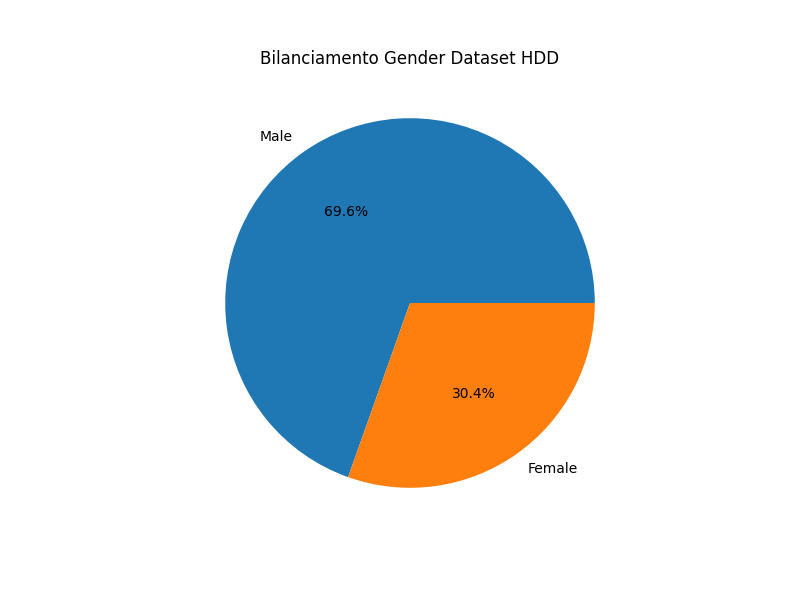
\includegraphics[width=0.75\linewidth]{TemplateTesi//immagini/tortaHDDsex.png}
    \caption{Grafico a Torta Relativo alla Feature 'Sex' in HDD}
    \label{fig:tortaHDDsex}
\end{figure}

\begin{flushleft}
    
Heart Disease Dataset (HDD) si presenta come un dataset abbastanza bilanciato, in quanto il numero di istanze rappresentanti i diversi valori della feature target  ($Heart\_Disease$) sono molto simili tra loro ( come visibile in figura \ref{fig:istoHDDtarget}).

La figura \ref{fig:tortaHDDsex} ci indica  la presenza di un bias nei dati, il numero di pazienti appartenenti al genere femminile è significativamente inferiore a quello di sesso maschile.
Nonostante ciò HDD è il dataset,tra quelli  clinici ,che presenta il maggiore numero di record (figura \ref{fig:datasets}).

\subsubsection{UCI}

\begin{figure}[H]
    \centering
    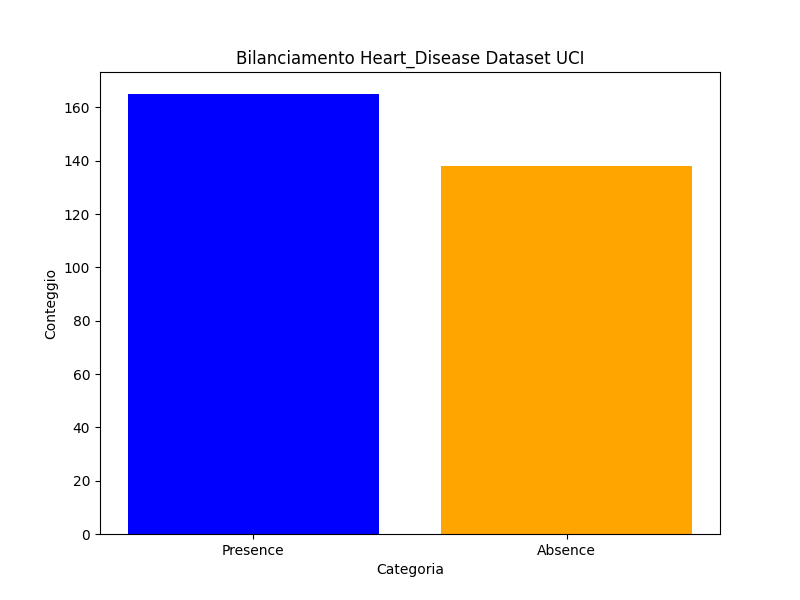
\includegraphics[width=0.75\linewidth]{TemplateTesi//immagini/istoUCItarget.png}
    \caption{Istogramma Relativo alla feature 'Heart\_Disease' in UCI}
    \label{fig:istoUCItarget}
\end{figure}
\begin{figure}[H]
    \centering
    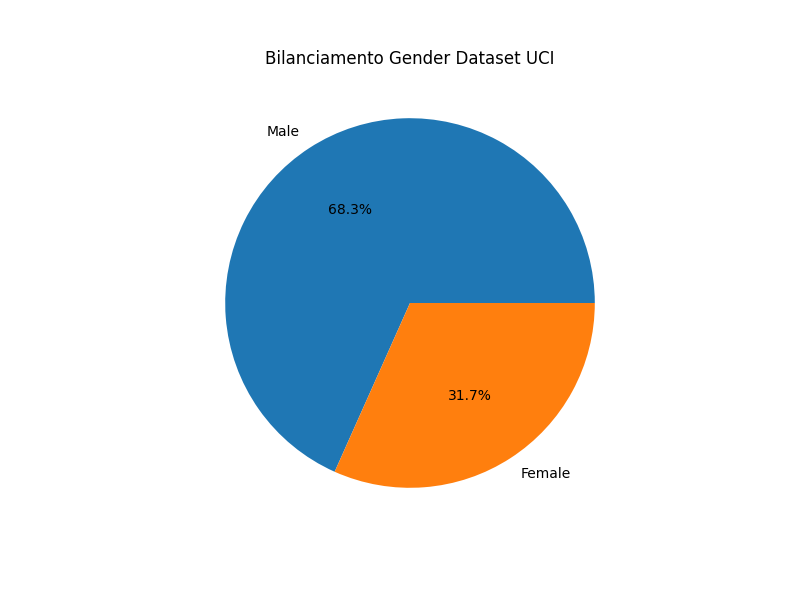
\includegraphics[width=0.75\linewidth]{TemplateTesi//immagini/tortaUCIsex.png}
    \caption{Grafico a Torta Relativo alla feature 'Sex' in UCI}
    \label{fig:tortaUCIsex}
\end{figure}
Come HDD il dataset UCI presenta un buon bilanciamento della feature target ma uno sbilanciamento nella rappresentazione del genere.

\subsubsection{PKI}


  \begin{figure}[H]
    \centering
    \includegraphics[width=0.75\linewidth]{TemplateTesi//immagini/istoPKItarget.png}
    \caption{Istogramma Relativo alla Feature 'Heart\_Disease' in PKI}
    \label{fig:istoPKItarget}
\end{figure}

\begin{figure}[H]
    \centering
    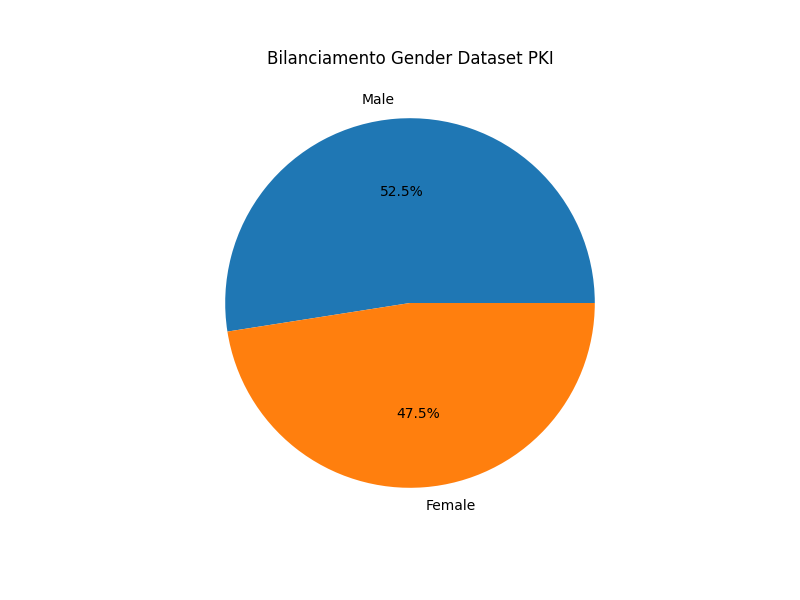
\includegraphics[width=0.75\linewidth]{TemplateTesi//immagini/tortaPKIsex.png}
    \caption{Grafico a Torta Relativo alla Feature 'Sex' in PKI}
    \label{fig:tortaPKIsex}
\end{figure}
Sebbene non presenti bias nella rappresentazione dei sessi all'interno dei dati (visibile in figura \ref{fig:istoPKItarget}) PKI possiede un forte sbilanciamento dei valori della feature "Heart\_Disease" (Questa problematica verrà successivamente trattata). 
È stato importante notare durante la fase esplorativa quali fossero i comportamenti dei valori delle features 'Personali' di PKI e se ci fossero alcune di queste particolarmente sbilanciate.
Tra queste ritengo importante segnalare la feature 'Etnia' (figura \ref{fig:EtniaPKI}), dove osserviamo uno sbilanciamento significativo della presenza di pazienti di etnia caucasica rispetto alle altre.
\begin{figure}[H]
    \centering
    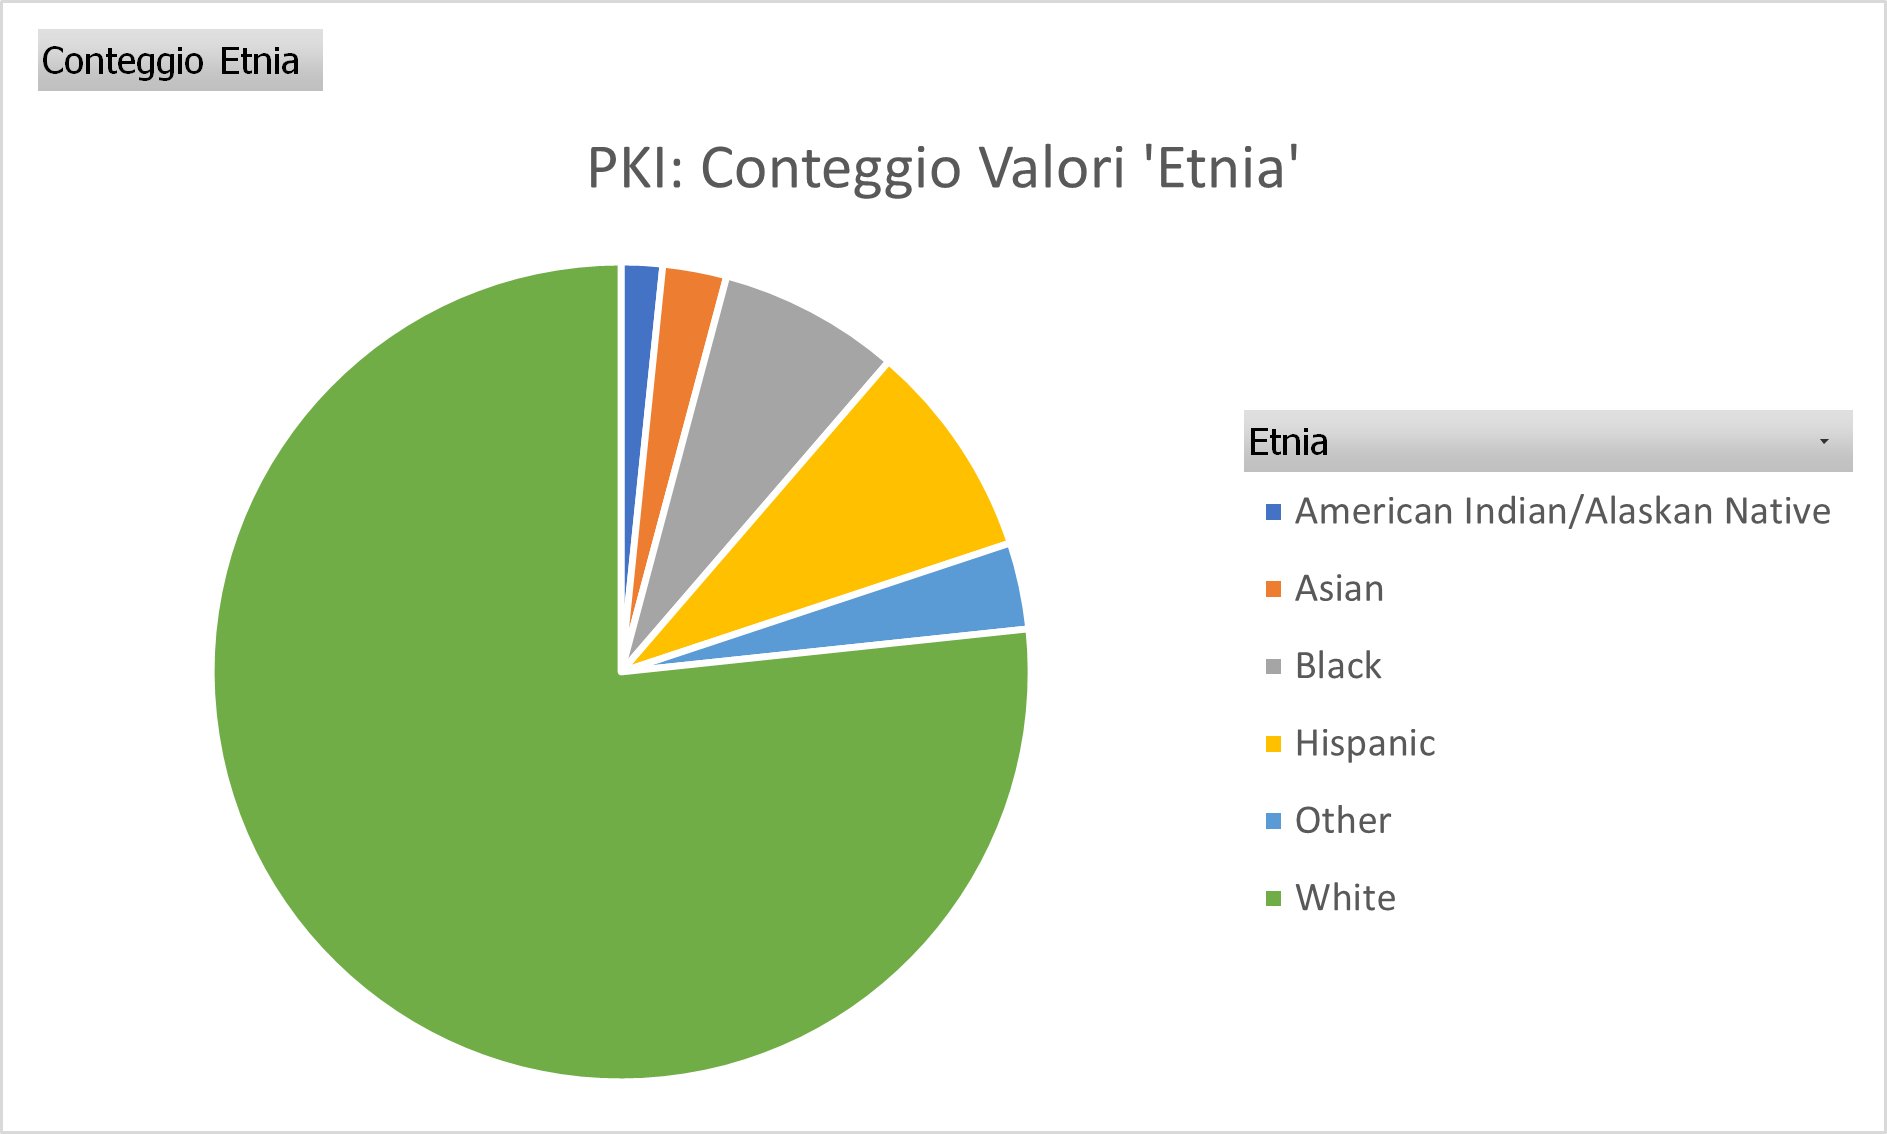
\includegraphics[width=0.75\linewidth]{TemplateTesi//immagini/EtniaRapp.png}
    \caption{Valori della feature categorica che descrive l'etnia di appartenenza dei partecipanti al sondaggio per la costruzione di PKI}
    \label{fig:EtniaPKI}
\end{figure}
\end{flushleft}

\begin{flushleft}
    
Durante la raccolta dei dati è importante cercare di bilanciare la rappresentazione sia dei sessi che dell'etnia.
Un Dataset completo e bilanciato aiuta sensibilmente a garantire la qualità dei risultati generati.
\end{flushleft}

\subsection{Distribuzioni delle feature nei Dataset \label{distribuzionisub}}

Vengono mostrate le distribuzioni di probabilità per i pazienti che presentavano o meno malattie cardiache, rappresentati nel dataset con il valore della feature "Heart\_Disease" rispettivamente 0 e 1. In particolare, sono state selezionate le distribuzioni relative alle feature individuate come le più promettenti. Le distribuzioni presentate nelle figure sottostanti sono state scelte per il loro elevato potenziale discriminatorio, valutato insieme al personale clinico usando un confronto \emph{qualitativo} delle distribuzioni in presenza o assenza di CVD nei pazienti.  
Tutto ciò è fondamentale durante l'allenamento del modello e per ottenere una previsione più accurata.

Nei seguenti grafici, sull'asse x sono riportati i valori delle specifiche feature, che possono essere sia categoriche che continue. Sull'asse y, invece, sono riportati i valori delle distribuzioni, sia per i casi di assenza che presenza di CVD, per facilitarne la comparazione.
\newline
\textbf{Distribuzioni HDD}
\newline



\begin{figure}[H]
    \centering
    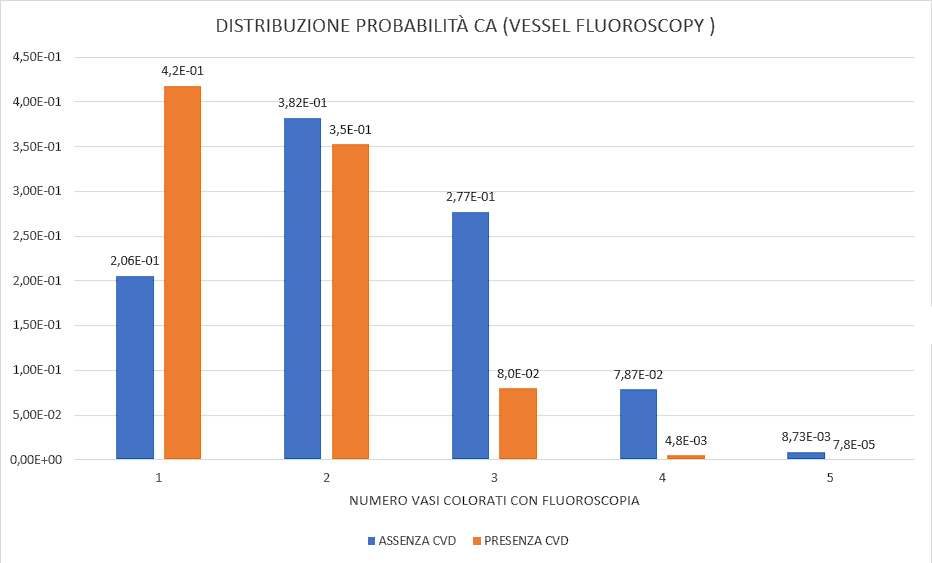
\includegraphics[width=1\linewidth]{TemplateTesi//immagini/CA.png}
    \caption{Distribuzioni di probabilità Fluoroscopia}
    \label{fig:dpHDDfluoro}
\end{figure}

\begin{figure}[H]
    \centering
    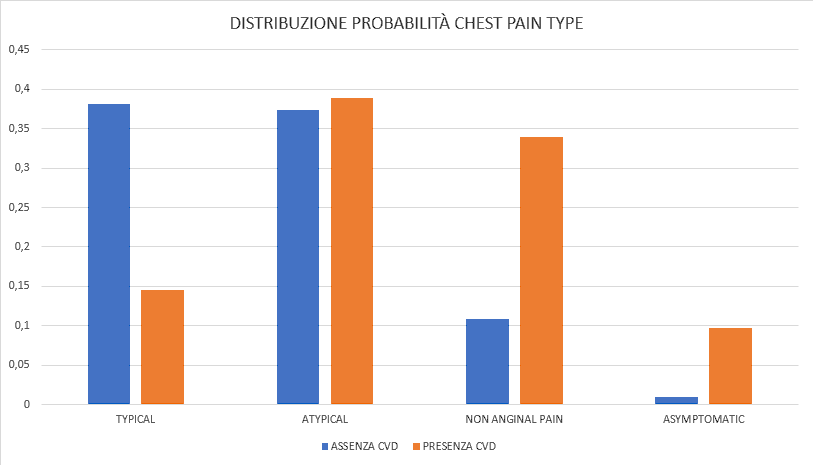
\includegraphics[width=1\linewidth]{TemplateTesi//immagini/CHEPAIN.png}
    \caption{Distribuzioni di probabilità Chest Pain Type}
    \label{fig:dpHDDchepain}
\end{figure}

\begin{figure}[H]
    \centering
    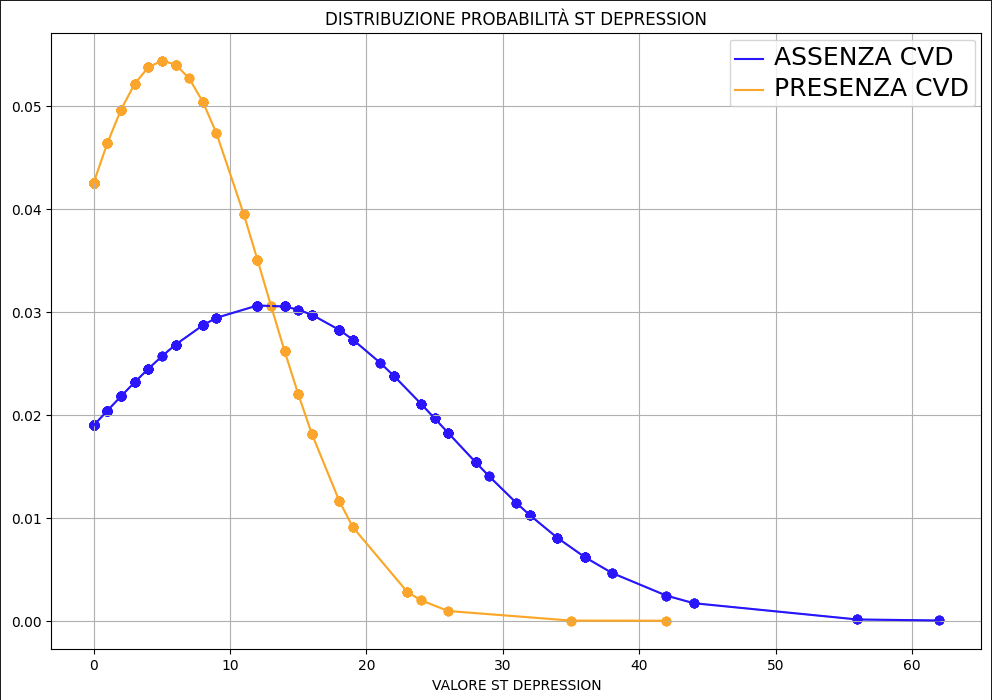
\includegraphics[width=1\linewidth]{TemplateTesi//immagini/stdepre.png}
    \caption{Distribuzioni di probabilità ST depression}
    \label{fig:dpHDDstdepre}
\end{figure}

\begin{figure}[H]
    \centering
    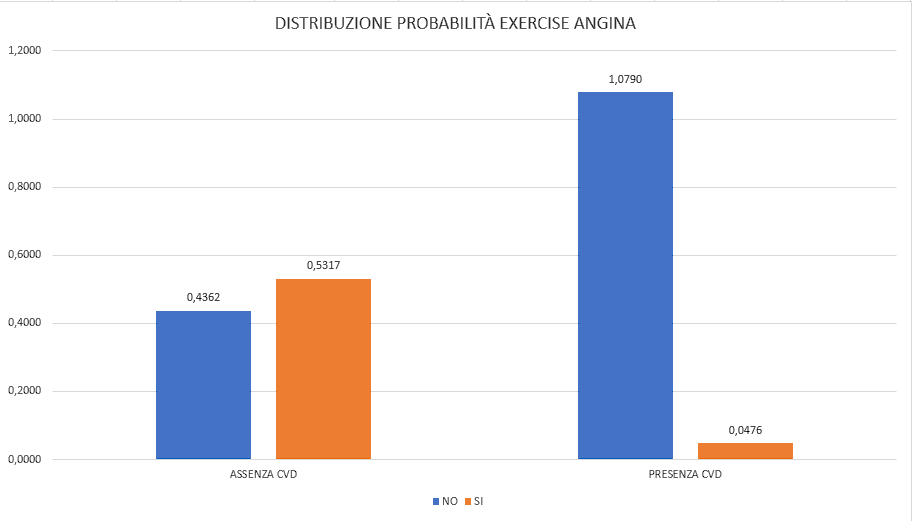
\includegraphics[width=1\linewidth]{TemplateTesi//immagini/EXECANGINA.png}
    \caption{Distribuzioni di probabilità Exercise Angina}
    \label{fig:dpHDDanginaexe}
\end{figure}



\begin{figure}[H]
    \centering
    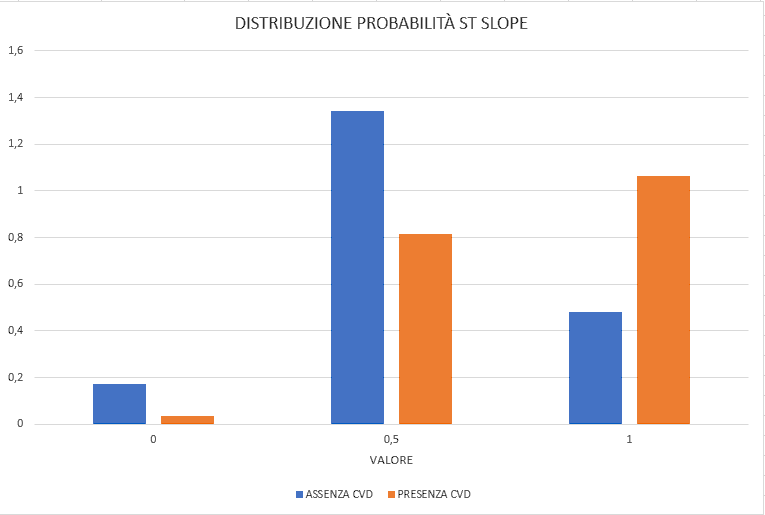
\includegraphics[width=1\linewidth]{TemplateTesi//immagini/SLOPE.png}
    \caption{Distribuzioni di probabilità ST Slope}
    \label{fig:dpHDDSlope}
\end{figure}
\newline
\textbf{Distribuzioni Personal Key Indicator of Heart Disease}
\newline

\begin{figure}[H]
    \centering
    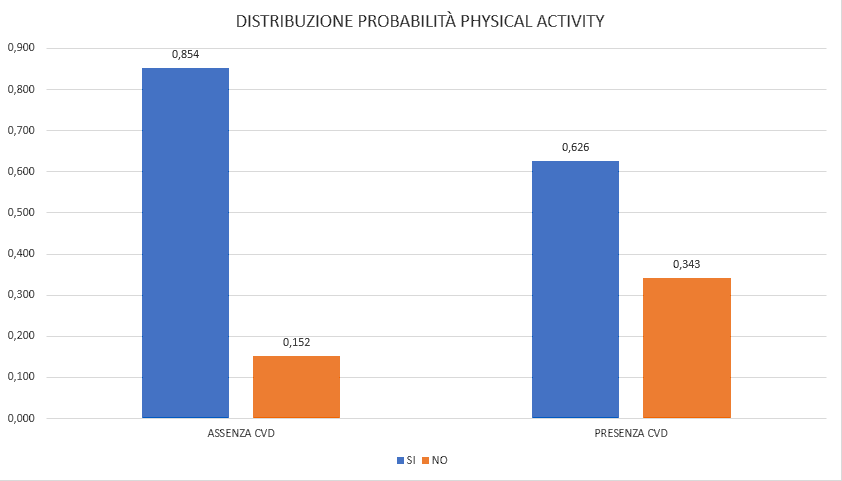
\includegraphics[width=1\linewidth]{TemplateTesi//immagini/PHYACTIVITY.png}
    \caption{Distribuzioni di Probabilità Physical Activity}
    \label{fig:dpPKIphyact}
\end{figure}


\begin{figure}[H]
    \centering
    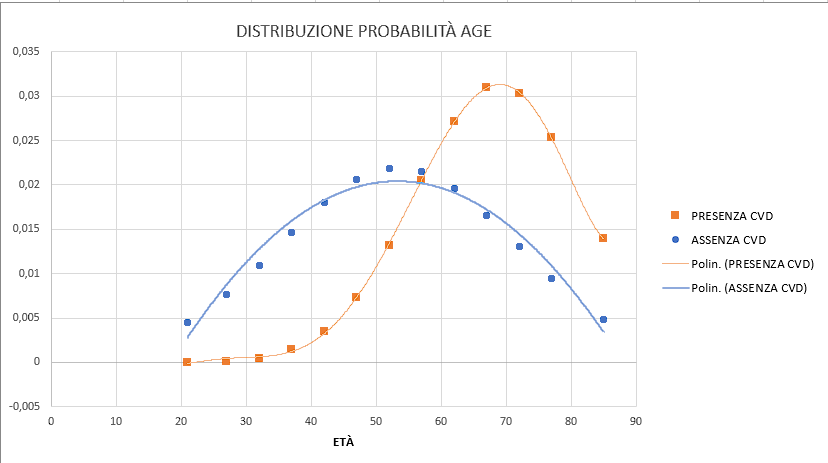
\includegraphics[width=1\linewidth]{TemplateTesi//immagini/AGE.png}
    \caption{Distribuzioni di Probabilità Age}
    \label{fig:dpPKIAge}
\end{figure}
\begin{figure}[H]
    \centering
    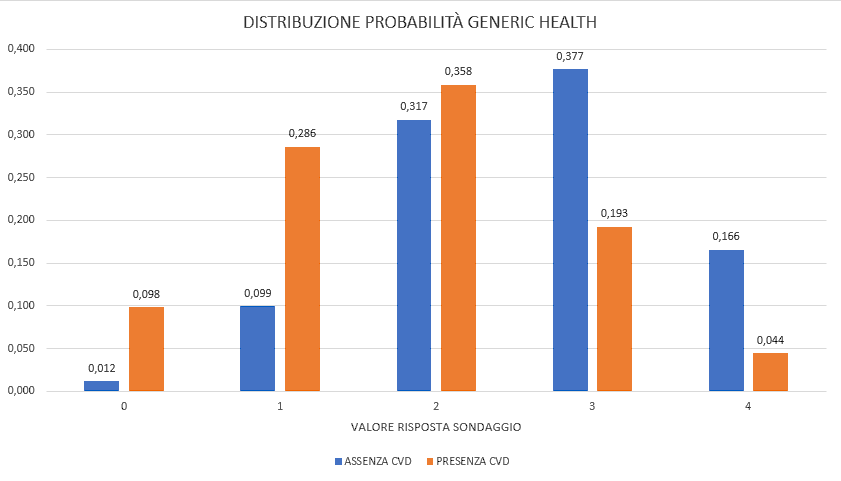
\includegraphics[width=1\linewidth]{TemplateTesi//immagini/GENHEALTH.png}
    \caption{Distribuzioni di Probabilità Generic Health}
    \label{fig:dpPKIGenhealth}
\end{figure}

\begin{figure}[H]
    \centering
    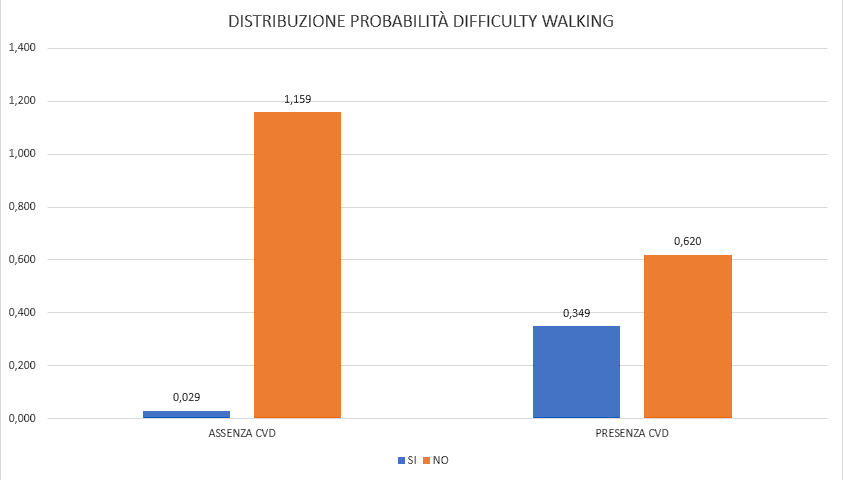
\includegraphics[width=1\linewidth]{TemplateTesi//immagini/DIFFWALK.png}
    \caption{Distribuzioni di Probabilità Difficulty Walking}
    \label{fig:dpPKIdiffwalk}
\end{figure}

\begin{figure}[H]
    \centering
    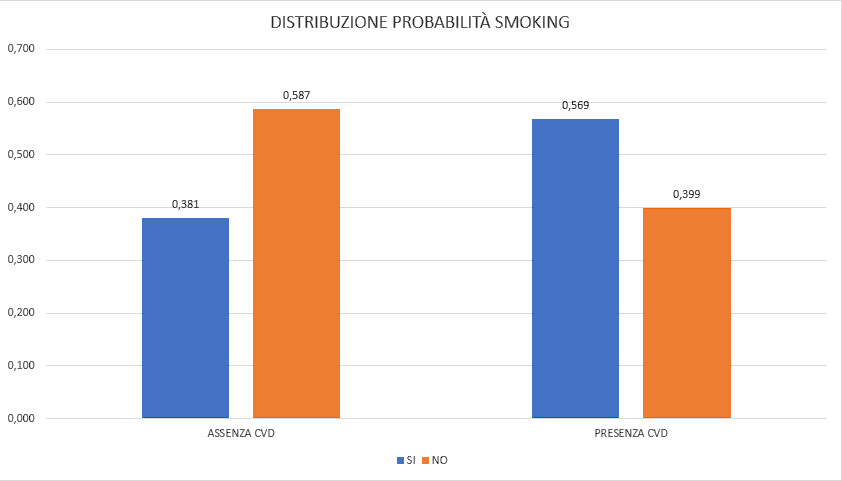
\includegraphics[width=1\linewidth]{TemplateTesi//immagini/SMOKING.png}
    \caption{Distribuzioni di Probabilità SMOKING}
    \label{fig:dpPKISMOKING}
\end{figure}

\begin{figure}[H]
    \centering
    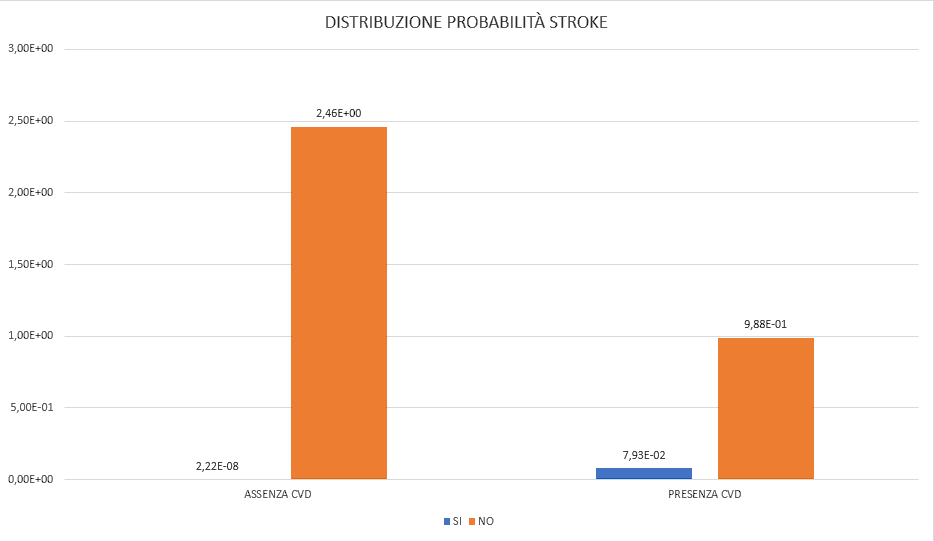
\includegraphics[width=1\linewidth]{TemplateTesi//immagini/stroke.png}
    \caption{Distribuzioni di Probabilità  Stroke}
    \label{fig:dpPKIStroke}
\end{figure}
\begin{figure}[H]
    \centering
    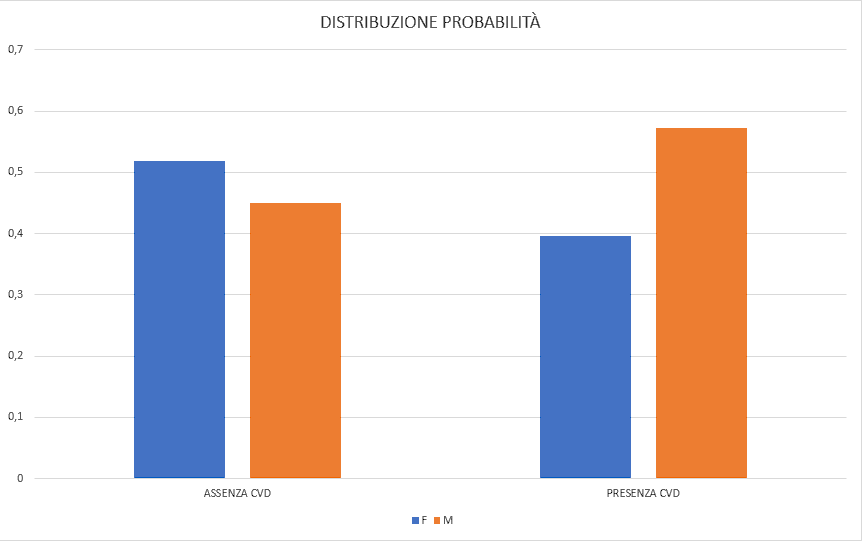
\includegraphics[width=1\linewidth]{TemplateTesi//immagini/sex.png}
    \caption{Distribuzioni di Probabilità Sex}
    \label{fig:dpPKISex}
\end{figure}
Le distribuzioni in cui il caso di assenza o presenza di malattia sono molto simili, come nel caso della feature "SleepTime" del dataset PKI illustrato nella Figura \ref{fig:sleeptime}, sono state classificate come distribuzioni con un apporto poco significativo.
\begin{figure}[H]
    \centering
    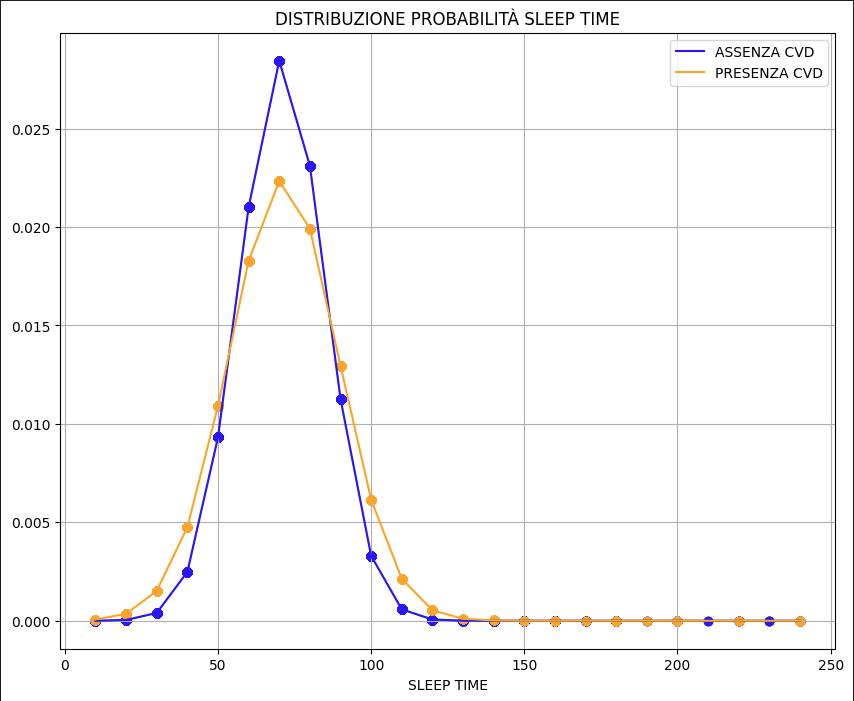
\includegraphics[width=0.7\linewidth]{TemplateTesi//immagini/sleeptime.png}
    \caption{Distribuzione della feature "Sleep Time"}
    \label{fig:sleeptime}
\end{figure}


\subsubsection{Considerazioni}
\begin{flushleft}
    
Un aspetto significativo che emerge dall'analisi delle distribuzioni dei valori delle feature nei due dataset è un aumento dell'incidenza delle malattie cardiache con l'avanzamento dell'età, con un picco intorno ai 68 anni. Questo dato indica che l'età rappresenta un fattore determinante nel predisporre gli individui alla comparsa di tali patologie. 
Inoltre, si è osservata una probabilità più alta di malattie cardiache tra i fumatori. Questo risultato sottolinea l'importanza del fumo come fattore di rischio per le patologie cardiache e l'urgenza di promuovere un interruzione del tabagismo e di sensibilizzazione verso uno stile di vita sano.

Una delle correlazioni rilevanti è stata riscontrata tra il sesso maschile e l'incidenza più elevata di patologie cardiache. Ciò suggerisce che il sesso può influenzare la suscettibilità alle stesse, richiedendo un'attenzione particolare nella valutazione delle condizioni del cuore nei soggetti di sesso maschile.

Un fattore importante che è emerso è la forte correlazione tra le difficoltà deambulatorie e l'incidenza di CVD. Questo implica che i problemi di mobilità possono essere considerati come possibili indicatori di patologie in tale ambito.
In assenza di malattie cardiache, è estremamente più probabile non aver avuto un infarto. Questo collegamento è intuitivo, poiché la presenza di un infarto suggerisce un precedente danno al cuore, aumentando la probabilità di sviluppare malattie cardiache, è stato quindi importante trovare tale riscontro nei dati.

Infine, come era prevedibile, l'attività fisica contribuisce alla riduzione dell'insorgenza di tali problematiche. Questo sottolinea l'importanza dell'esercizio fisico regolare e dell'adozione di uno stile di vita attivo per la prevenzione delle CVD.
\end{flushleft}


\subsection{Analisi dei Coefficienti di Correlazione}

Si riportano per i dataset PKI e HDD
le heatmap dei coefficienti di correlazione generate




%\subsubsection{HeatMap Personal Key Indicator of Heart Disease}

\begin{figure}[H]
    \centering
    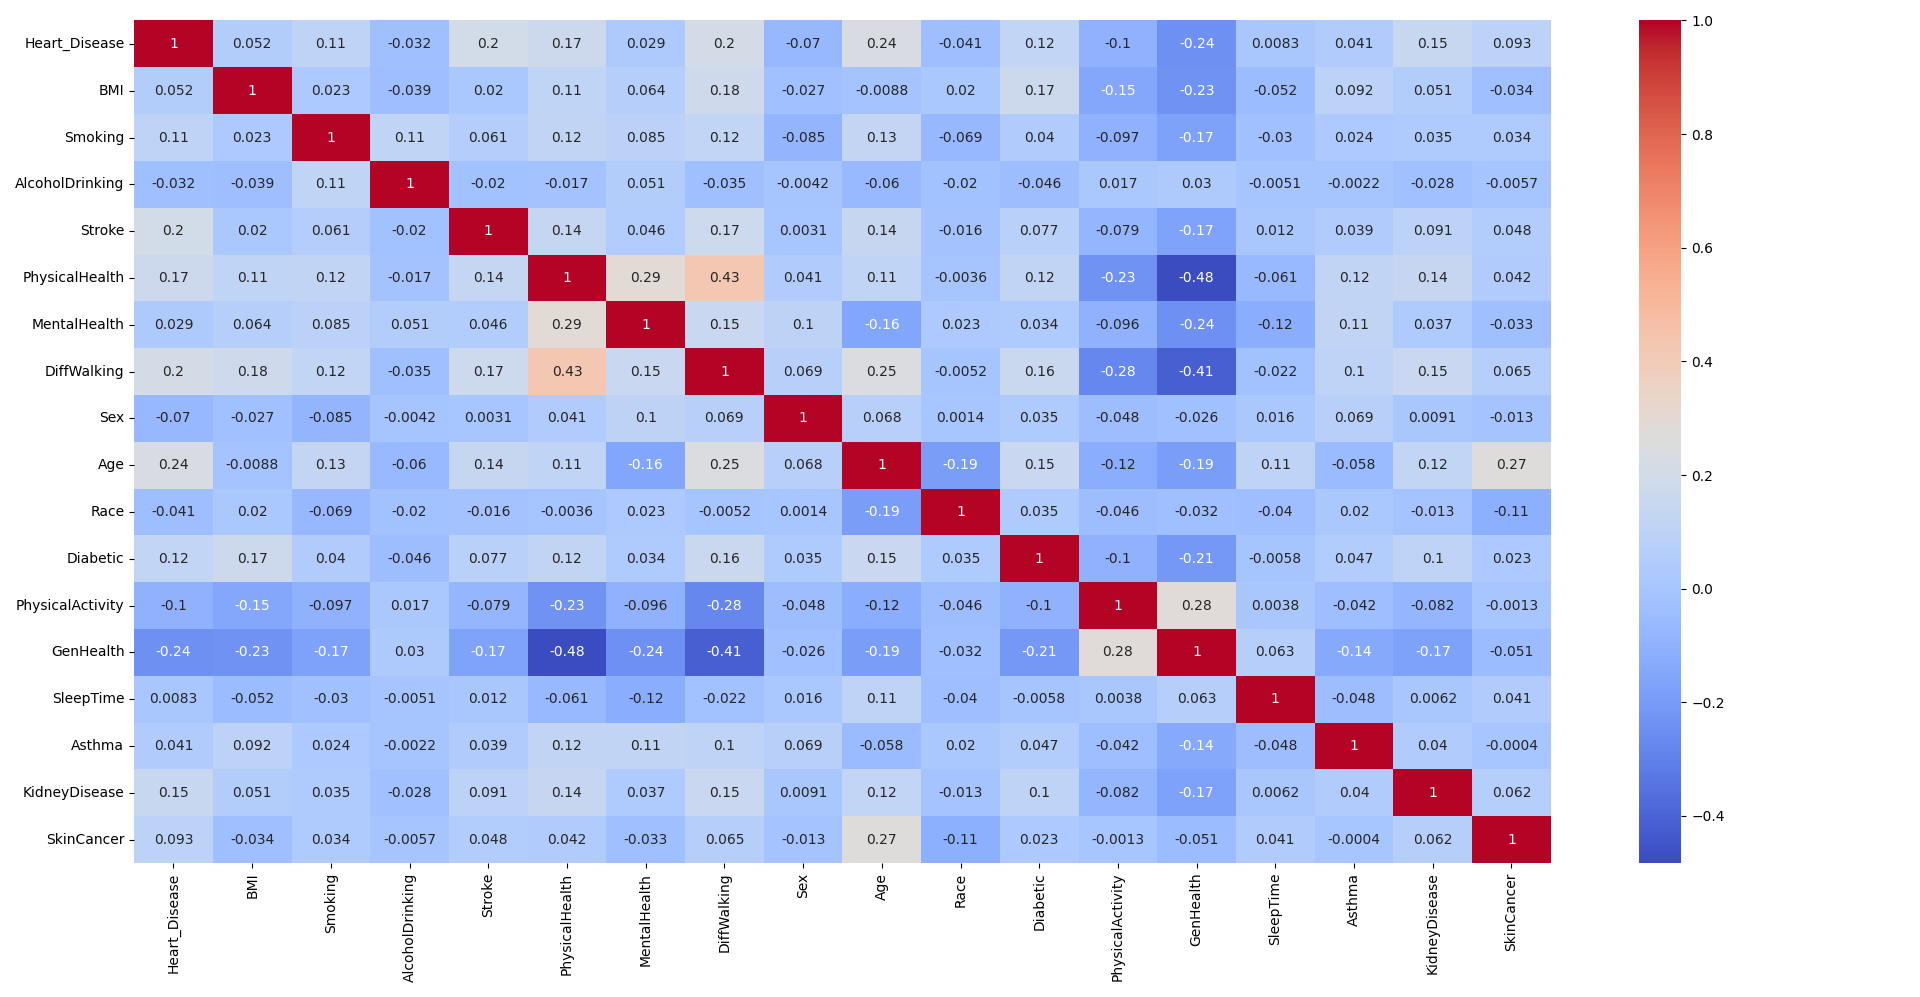
\includegraphics[width=1\linewidth]{TemplateTesi//immagini/heatmappki2.png}
    \caption{HeatMap dei coefficienti di correlazione di PKI}
    \label{fig:corrPKI}
\end{figure}


\begin{figure}[H]
    \centering
    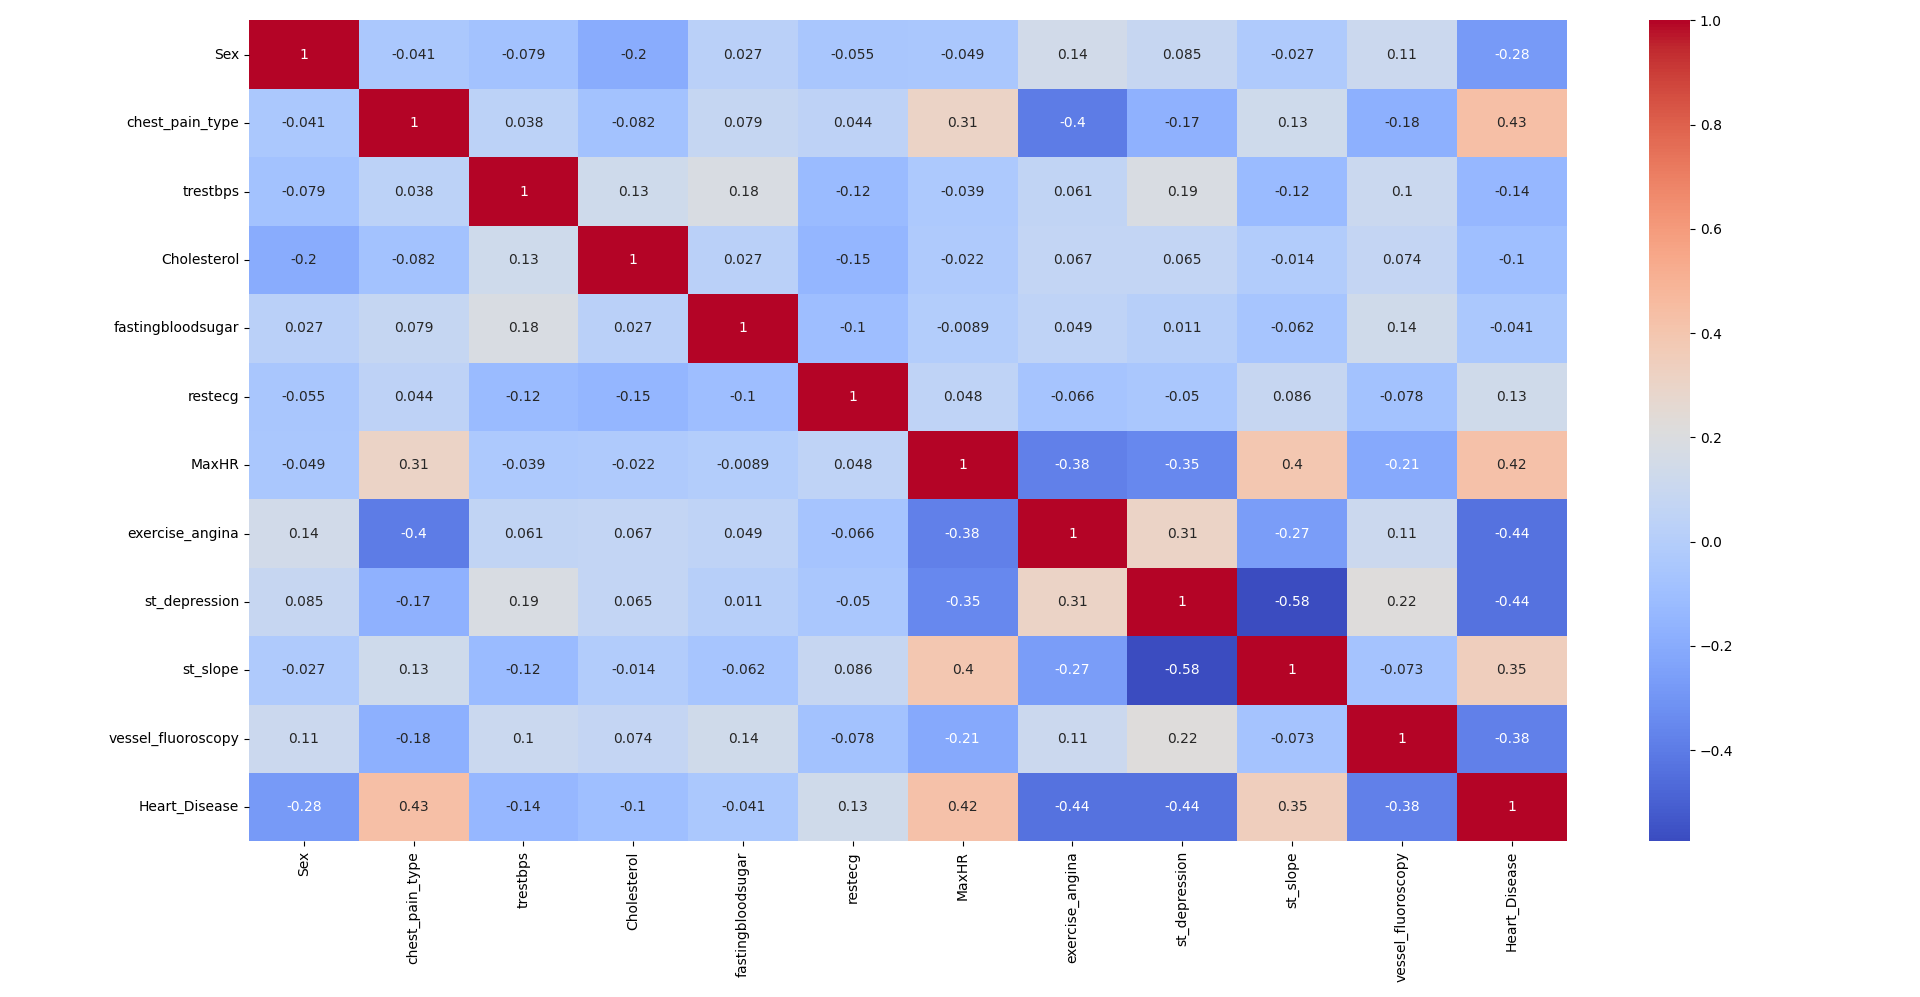
\includegraphics[width=1.1\linewidth]{TemplateTesi//immagini/heatmapHDD.png}
    \caption{HeatMap dei coefficienti di correlazione di HDD }
    \label{fig:corrHDD}
\end{figure}




%\subsubsection{Considerazioni}
In generale, sebbene non siano stati riscontrati coefficienti di correlazione estremamente alti, i risultati sotto riportati sono comunque significativi e offrono un'importante rappresentazione delle relazioni tra le variabili considerate nei dataset. 
\begin{flushleft}
    
\newline
\textbf{PKI}
\newline
Uno dei risultati significativi emersi dai risultati in figura \ref{fig:corrPKI} è la correlazione  tra la difficoltà nel camminare (Difficulty walking) e la salute generica(Generic Health). Questo implica che vi sia una connessione rilevante tra l'abilità motoria di una persona e il suo stato di salute generale. Tale risultato potrebbe indicare l'importanza di monitorare attentamente la difficoltà nel camminare al fine di valutare e intervenire  per migliorare la propria salute generale.

Inoltre, risulta una correlazione tra la salute fisica (Physical Health) e la salute generale (Generic Health). Questo suggerisce che il benessere fisico di una persona può influire significativamente sulla sua salute generica.

Infine, si è  osservato una correlazione tra la salute fisica (Physical Health) e la difficoltà nel camminare (Difficulty walking). Questo risultato mette in evidenza come il livello di benessere fisico influenzi le capacità deambulatorie delle persone. L'identificazione di tale relazione potrebbe avere implicazioni nella progettazione della riabilitazione.
\newline
\textbf{HDD}
\newline
Uno dei risultati più significativi in figura \ref{fig:corrHDD} riguarda la buona correlazione tra St slope e St depression. 
È ragionevole riconoscere questa connessione in quanto entrambe le caratteristiche sono strettamente legate all'analisi clinica del tratto ST \cite{stsegment}dell'elettrocardiogramma.

È stata osservata una correlazione tra la ST depression e la presenza di malattie cardiache (Heart Disease). Ciò suggerisce che la depressione del tratto ST potrebbe essere un fattore importante nella valutazione della presenza o dello sviluppo di malattie cardiache. 

Inoltre, si riscontra una correlazione  tra la tipologia di dolore toracico (Chest Pain Type) e la presenza di CVD. Questo suggerisce che il tipo di dolore toracico riportato da un individuo può essere indicativo della presenza o dello sviluppo di problematiche al cuore.

Altri risultati significativi includono la correlazione tra il battito cardiaco massimo raggiunto (MAX Heart Rate) e la presenza di malattie cardiache, nonché la correlazione  tra l'angina indotta dall'esercizio fisico (Exercise Angina) e il tipo di dolore toracico con queste ultime. Questi risultati sottolineano l'importanza di tali variabili nella valutazione della salute del cuore e possono fornire utili indizi per la diagnosi e la gestione delle CVD.
\end{flushleft}


\subsection{MIScore dei Datasets}
Si riportano per i due dataset principali i MiScore calcolati per varie feature.

\begin{figure}[H]
    \centering
    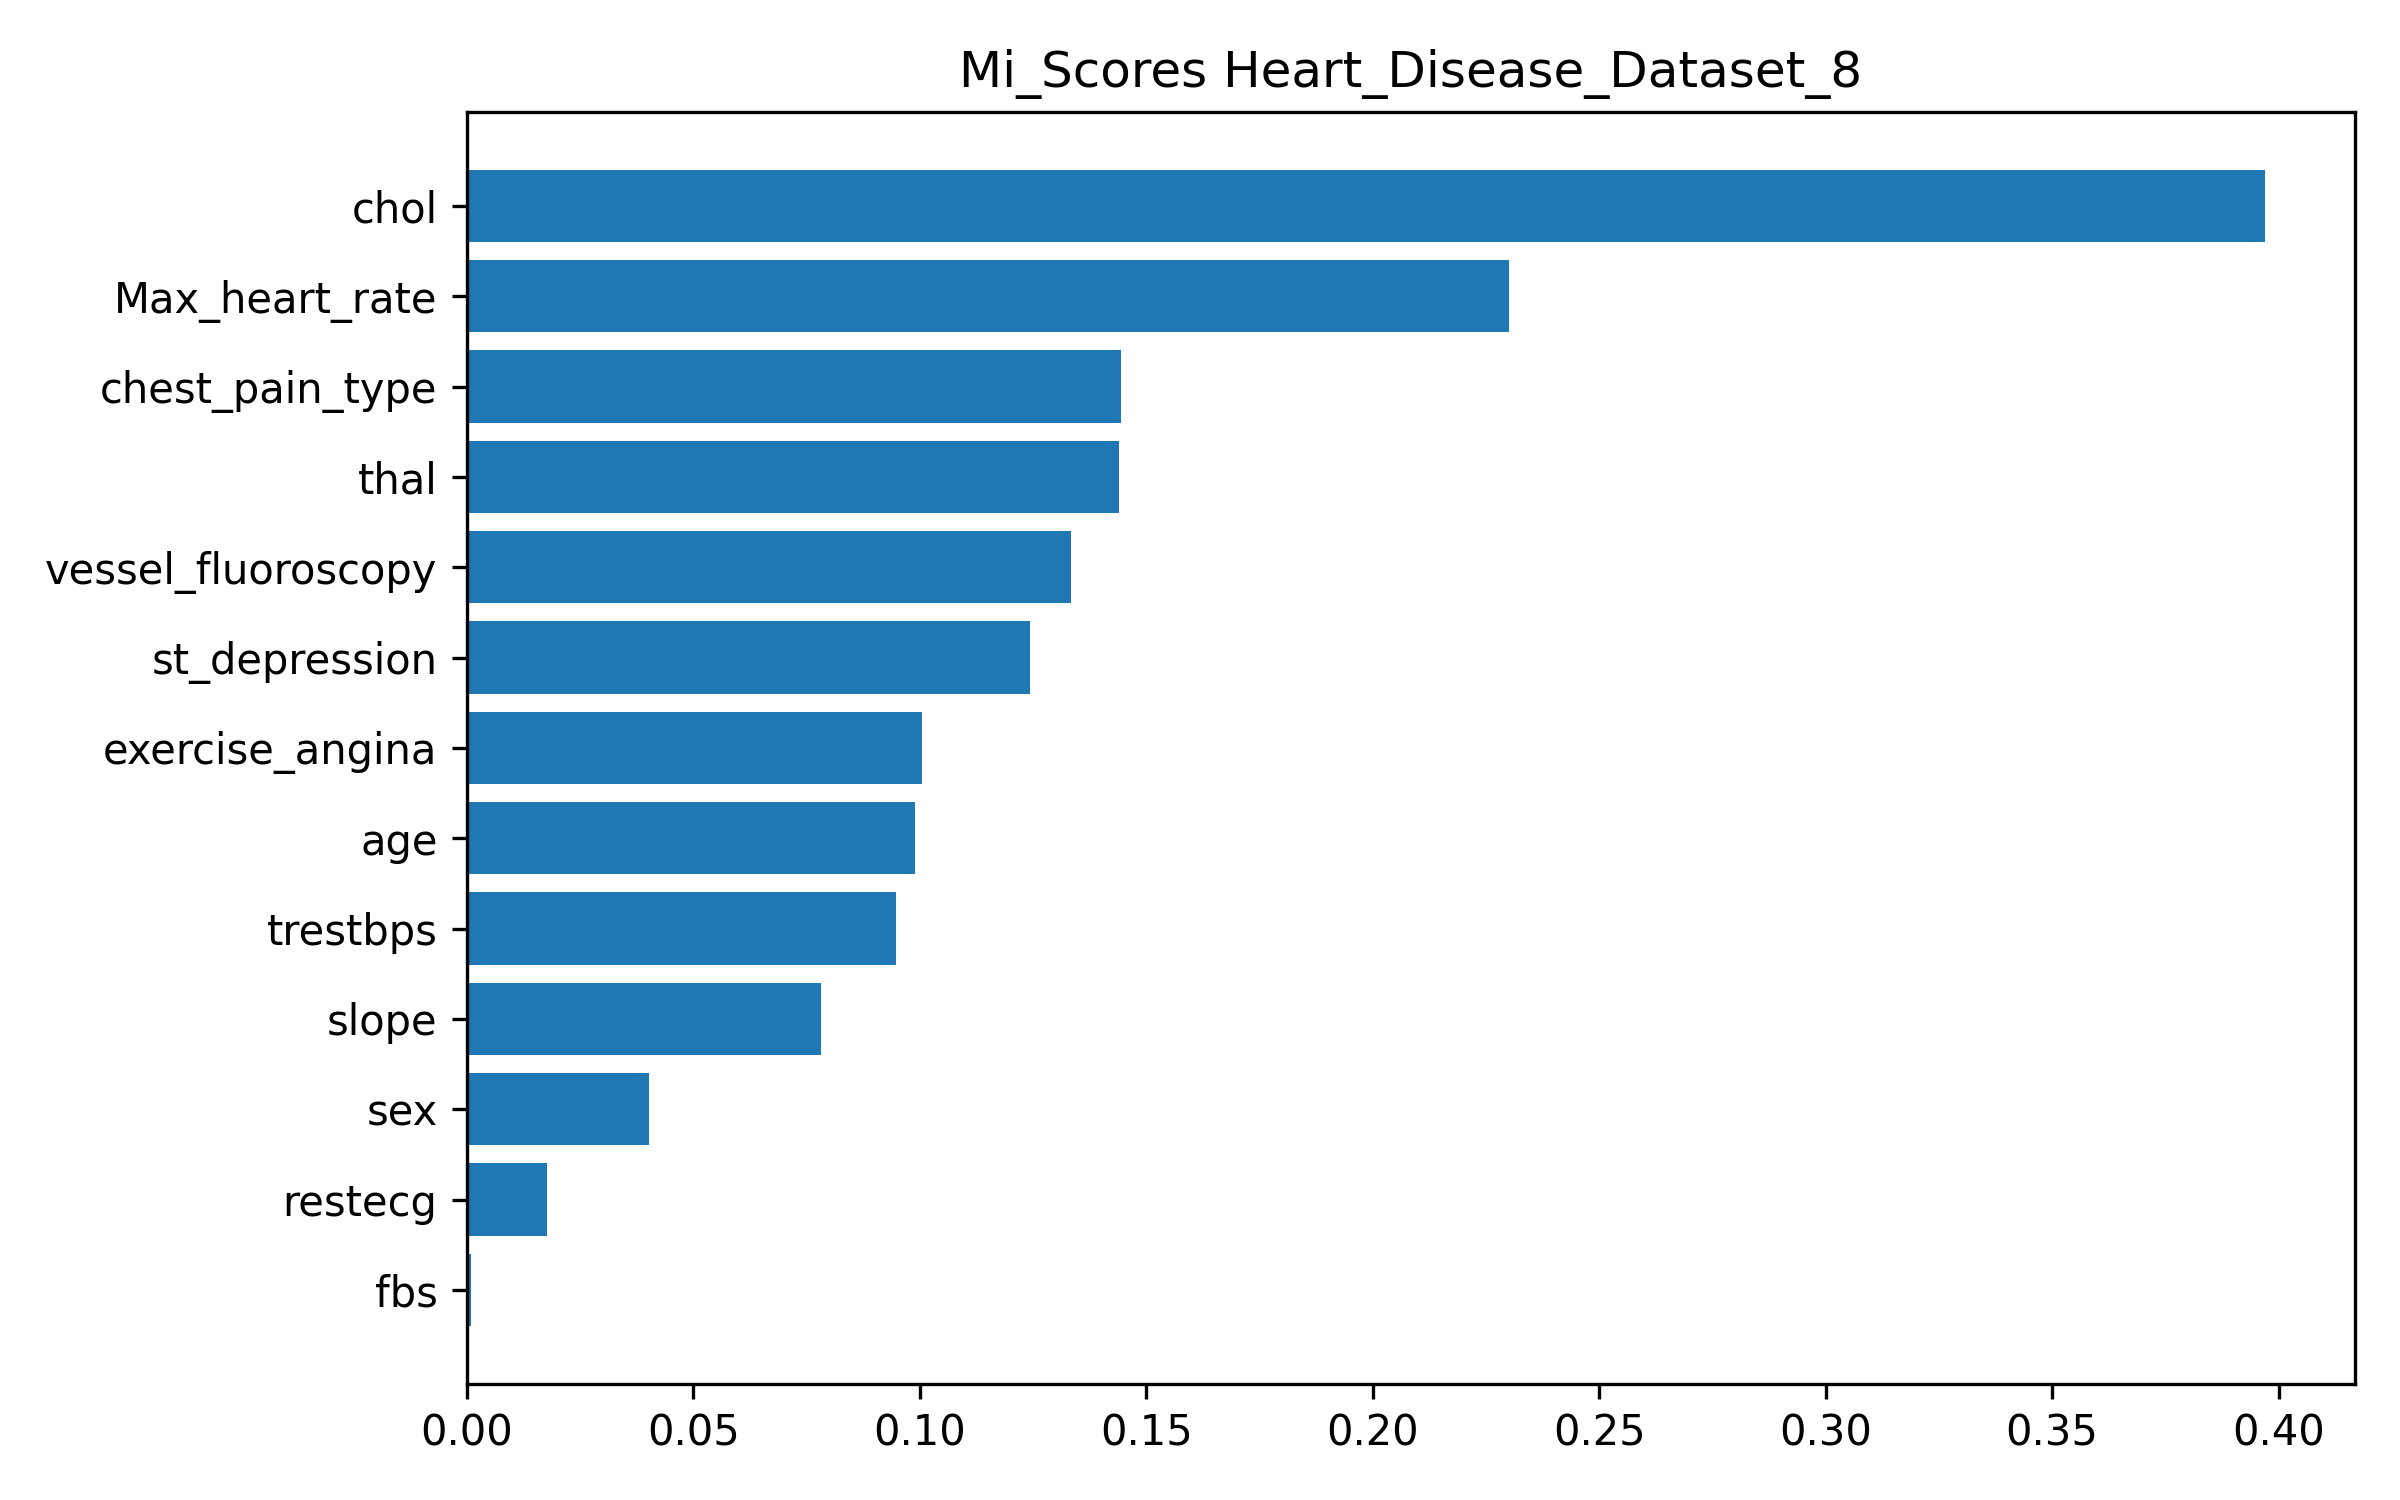
\includegraphics[width=1\linewidth]{TemplateTesi//immagini/Heart_Disease_Dataset_8_mi_score.png}
    \caption{MIScore calcolati per HDD}
    \label{fig:miscorehdd}
\end{figure}



\begin{figure}[H]
    \centering
    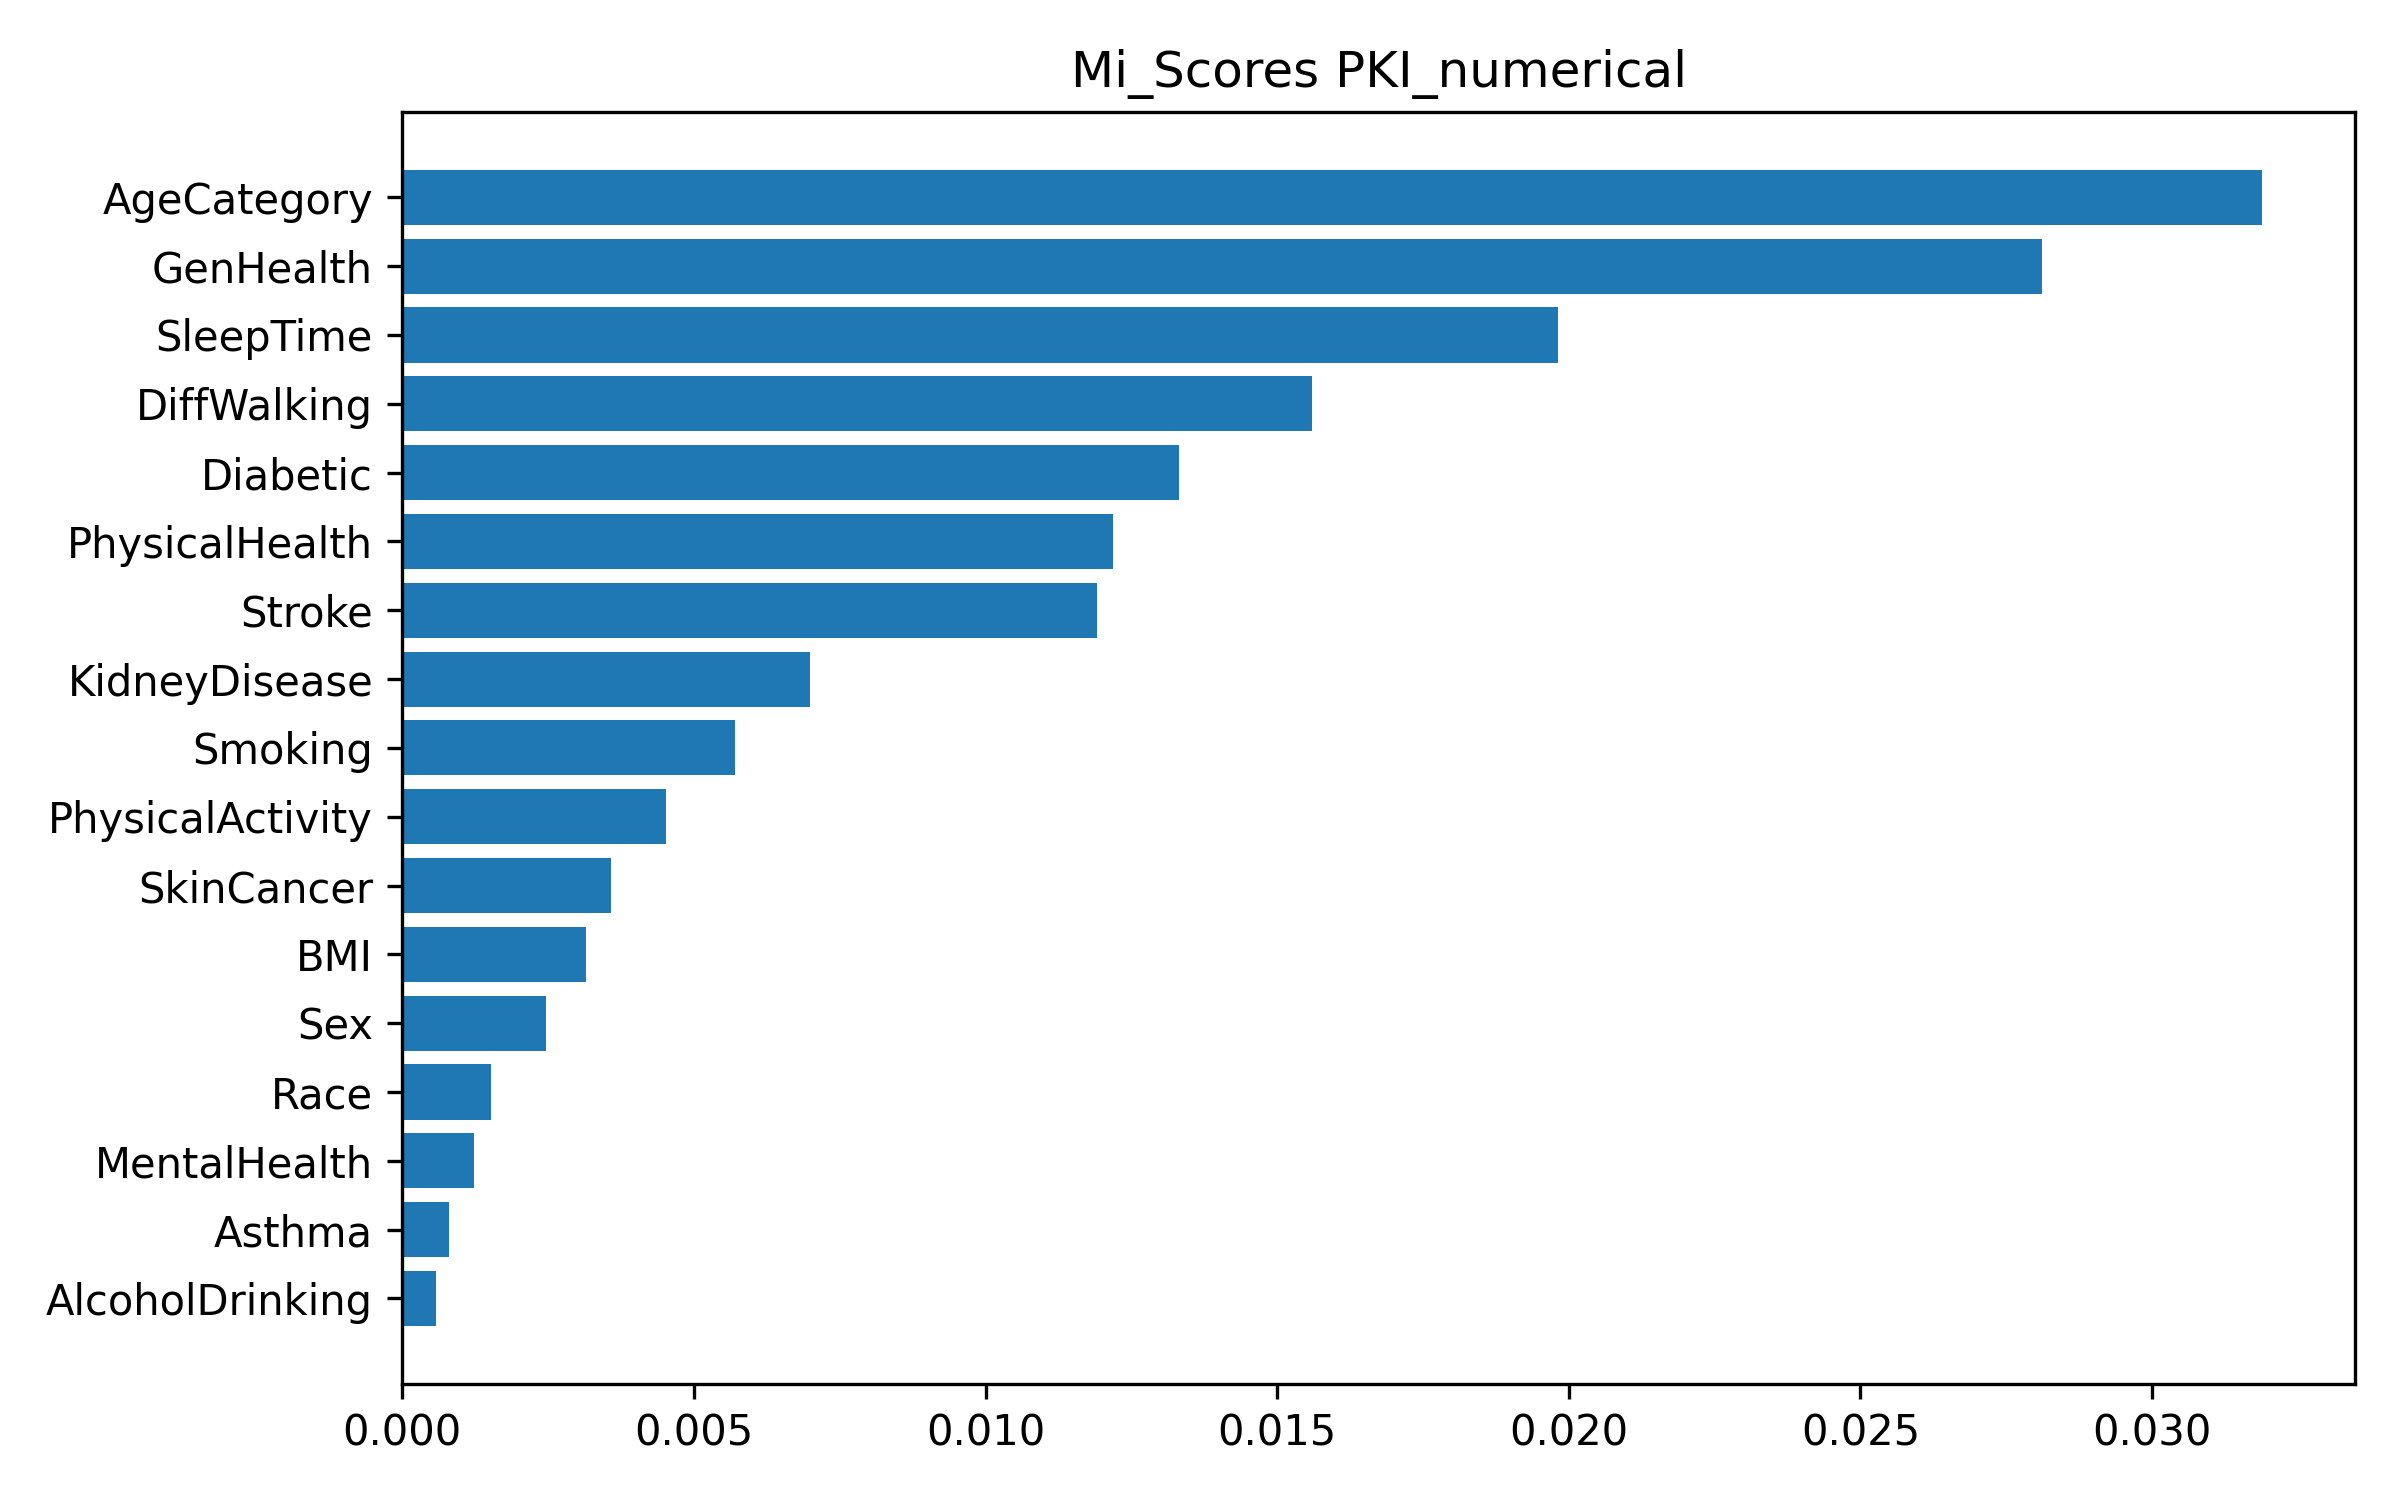
\includegraphics[width=1\linewidth]{TemplateTesi//immagini/PKI_numerical_mi_score.png}
    \caption{MIScore calcolati per PKI}
    \label{fig:miscorePKI}
\end{figure}


%\subsubsection{Considerazioni}

\textbf{PKI}
\begin{flushleft}
    
I risultati ottenuti dal grafico dei MI Score per il dataset PKI (in figura \ref{fig:miscorePKI}) hanno indicato che l'età (Age Category) si posiziona in cima alla lista delle feature più influenti per la classificazione delle CVD. Questo suggerisce che l'età può essere un fattore chiave nel determinare la presenza o l'assenza di tali patologie (In accordo con le considerazioni ottenute durante l'analisi qualitativa delle distribuzioni).


In seconda posizione nel grafico dei MI Score troviamo la salute generale (Generic Health). 
La correlazione tra la salute generale e la presenza di patologie cardiache suggerisce l'importanza di una valutazione completa delle condizioni di salute complessive per identificare  eventuali problematiche in ambito cardiovascolare.

Al terzo posto si colloca il tempo dedicato quotidianamente al sonno (Sleep Time). Questo risultato suggerisce che le abitudini e la qualità del sonno possono essere fattori rilevanti nella valutazione delle malattie cardiache, evidenziando l'importanza di uno stile di vita sano e un adeguato riposo per preservare la salute cardiovascolare \cite{sonnocvd}.
La difficoltà nel camminare (Difficulty Walking) si piazza al quarto posto nel grafico dei MI Score. Questo sviluppo sottolinea come le condizioni motorie siano legate alle malattie cardiache, suggerendo che i problemi di mobilità possono essere un segnale di allarme per ulteriori valutazioni cardiovascolari.

Le feature relative alla presenza di diabete (Diabetic) , l'etnia e genere (Sex) occupano invece posizioni meno rilevanti di quelle attese.
\newline


\textbf{HDD}
\newline
I risultati ottenuti dal grafico dei MI Score per il dataset HDD (figura \ref{fig:miscorehdd}) hanno rivelato che il colesterolo (Chol) occupa la prima posizione nella lista delle feature più influenti per la classificazione. Questo indica come i livelli di colesterolo possano essere un indicatore significativo per la valutazione delle patologie cardiovascolari, suggerendo l'importanza del monitoraggio di questo parametro nella prevenzione e riabilitazione nel contesto cardio.

Al secondo e terzo posto troviamo il battito cardiaco massimo raggiunto (Max Heart Rate) e la tipologia di dolore toracico (Chest Pain Type). Questi risultati ci forniscono dei parametri di tipo clinico da tenere di conto in fasi diagnostiche e riabilitative.

È interessante notare che l'età (Age) e il genere (Sex) occupano posizioni poco rilevanti nel grafico, nonostante la posizione prominente dell'età nel grafico precedente. 



\end{flushleft}





\subsection{Selezione feature iniziali}
\begin{flushleft}
    
Dopo aver svolto tali analisi e tratte le suddette considerazioni, sono stati combinati tali risultati per una prima selezione del set di feature da utilizzare per la creazione dei modelli.

Per identificare i primi set di feature  è stata inizialmente eseguita una cernita qualitativa delle distribuzioni delle stesse (come quelle riportate in \ref{distribuzionisub}).
Durante l'analisi manuale e qualitativa effettuata sono state selezionate le feature che sembravano avere una potenziale influenza significativa per la classificazione, basandomi anche sull'esperienza clinica della mia referente aziendale. Successivamente, sono stati confrontati i risultati di questa analisi sulle distribuzioni con quelli ottenuti dalle heatmap dei coefficienti di correlazione e dai grafici del MI Score.

Attraverso il confronto tra queste analisi, sono state individuate le feature che mostravano correlazioni o relazioni significative in tutte le analisi, andando a scegliere sia le feature che risultavano significative in tutte e tre le analisi contemporaneamente che quelle più promettenti delle singole analisi.  

Per il dataset PKI sono state quindi inizialmente scelte le seguenti features:

 \begin{lstlisting}
Chosen_Features=['Age','Sex','Smoking','PhysicalActivity','GenHealth','DiffWalking']
\end{lstlisting}

Per il dataset HDD:
\begin{lstlisting}
Chosen_Features=['Age', 'Sex', 'chest_pain_type', 'st_depression', 'st_slope', 'exercise_angina']
\end{lstlisting}


Il dataset UCI, invece, non ha volutamente ricevuto feature selection, sono state quindi selezionate tutte le feature:

\begin{lstlisting}
Chosen_Features=['Age', 'Sex', 'chest_pain_type', 'st_depression', 'st_slope', 'exercise_angina','trestbps','Cholesterol,'fasting_blood_sugar','MaxHR','exercise_angina','vessel_fluoroscopy']
\end{lstlisting}
		
\end{flushleft}

\section{Elaborazioni Successive}
\subsection{Scelta dei Modelli}
\begin{flushleft}
    
Nella presente sezione, si delinea la fase determinante della selezione del modello per la creazione del modello finale. Verranno presentati i risultati della valutazione dei modelli considerati nel contesto del nostro problema di ricerca. Sono stati scelti quattro modelli di ML (ADA,XGB,SVM,RF), ciascuno dei quali è stato addestrato e valutato mediante le tecniche illustrate nel capitolo precedente.

%\subsubsection{Risultati della Valutazione}

Di seguito, %due esempi di valutazione dei 
mostriamo i risultati ottenuti per il dataset HDD e PKI:
i valori mostrati sono stati calcolati durante la fase di esplorazione dei modelli,calcolati con solo l'utilizzo dei set di feature iniziali, e utilizzando gli iperparametri di default dei modelli.
I grafici \ref{fig:graficosceltamodello} e \ref{fig:graficosceltamodellopki}, ci mostrano i risultati ottenuti durante l'analisi.


    
    \begin{figure}[H]
        \centering
        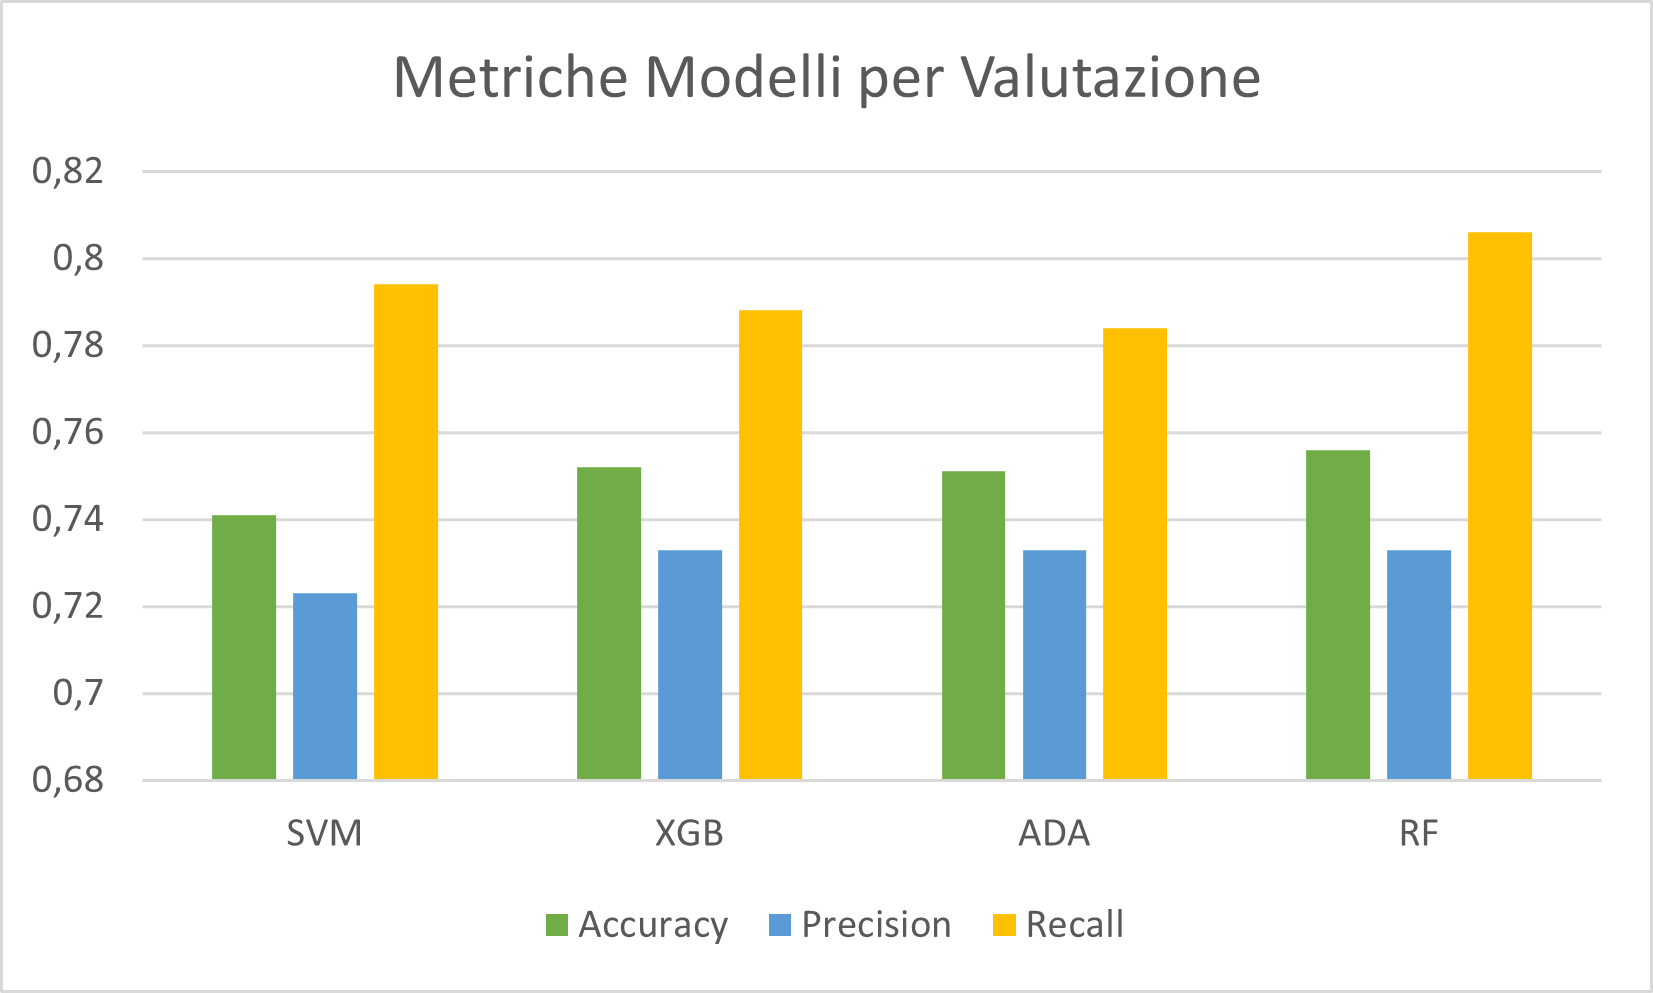
\includegraphics[width=0.75\linewidth]{TemplateTesi//immagini/GraficoComparazioneModelli.png}
        \caption{Valori delle metriche valutate per la scelta del modello finale per HDD.}
        \label{fig:graficosceltamodello}
    \end{figure}

\begin{figure}[H]
        \centering
        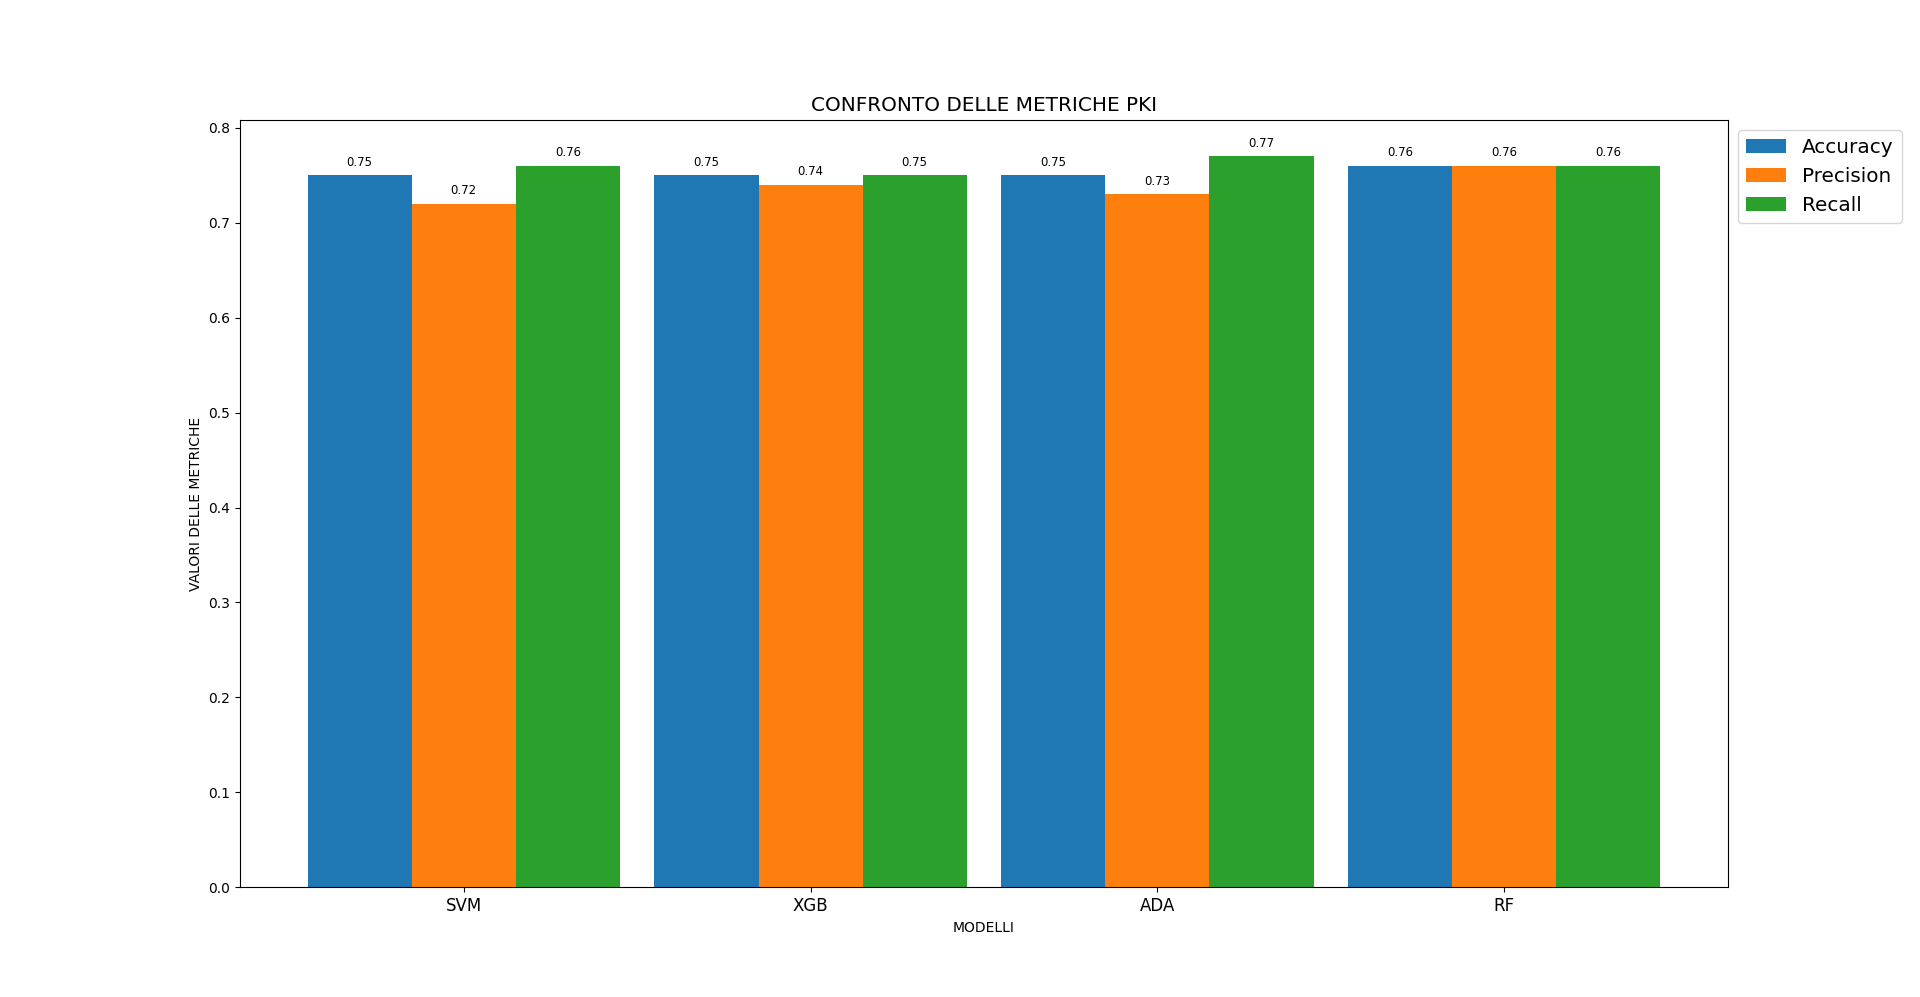
\includegraphics[width=1\linewidth]{TemplateTesi//immagini/metricheinizialipki.png}
        \caption{Valori delle metriche valutate per la scelta del modello finale per PKI.}
        \label{fig:graficosceltamodellopki}
    \end{figure}
Come anticipato nel capitolo 2, e come visibile dai grafici, Random Forest raggiunge risultati più stabili e generalmente migliori . Quindi presenteremo le analisi successive usando solo questo modello.

\end{flushleft}

\subsection{Feature Selection: esempio per PKI \label{selezionesetfinali}}
\begin{flushleft}
Durante l'analisi dei dataset, sono stati condotti dei test per identificare le feature più promettenti, oltre a quelle iniziali selezionate durante la fase di EDA, andando così a creare i set di feature finali per ogni modello. A tal proposito, saranno illustrati alcuni test effettuati sulle feature del dataset PKI, che consistono in aggiungere delle nuove feature e rivalutando la performance del modello RF. Dei test simili sono stati effettuati anche su HDD. 
\newline
Inizialmente per PKI, erano state selezionate le seguenti feature:
\emph{ChosenFeatures=[Age,Sex,Smoking,PhysicalActivity,GenHealth,DiffWalking]}
\newline
Successivamente, è stata valutata l'evoluzione delle metriche aggiungendo nuove features.
\subsubsection{Aggiunta di Physical Health}

\begin{figure}[H]
    \centering
    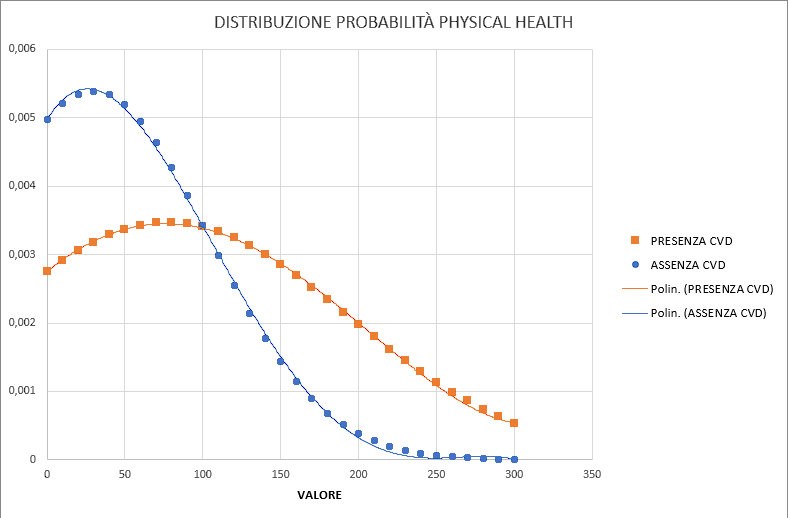
\includegraphics[width=1\linewidth]{TemplateTesi//immagini/PHYHEALTH.png}
    \caption{Distribuzione della Feature Physical Health in PKI}
    \label{fig:PHPKIDistr}
\end{figure}
Ho calcolato lo score delle metriche per 
\newline
\emph{ChosenFeatures=[Age,Sex,Smoking,PhysicalActivity,GenHealth,DiffWalking]}
\newline
ottenendo:
\begin{lstlisting}
'test_accuracy': array([0.75085106, 0.75871825, 0.75833272, 0.75674467, 0.75738354]), 
'test_precision': array([0.72459836, 0.73654873, 0.73590252, 0.73289951, 0.7355619 ]), 
'test_recall': array([0.80928738, 0.80558547, 0.80587398, 0.80793662, 0.80370181])}
\end{lstlisting}
Dopo aver inserito tra le features scelte 'PhysicalHealth', ottenendo così 
\newline
\emph{ChosenFeatures=[Age,Sex,Smoking,PhysicalActivity,GenHealth,DiffWalking,PhysicalHealth]}

I risultati ottenuti sulle metriche sono i seguenti:

\begin{lstlisting}
'test_accuracy': array([0.77163615, 0.78540917, 0.78433216, 0.78378255, 0.78447623]), 'test_precision': array([0.75491221, 0.76111427, 0.76292158, 0.76052892, 0.76504303]), 'test_recall': array([0.8044395 , 0.83193078, 0.82504883, 0.82840453, 0.82114237])
\end{lstlisting}

Ovvero un \emph{incremento globale di circa il 2\%}


\subsubsection{Aggiunta di SleepTime}
\begin{figure}[H]
    \centering
    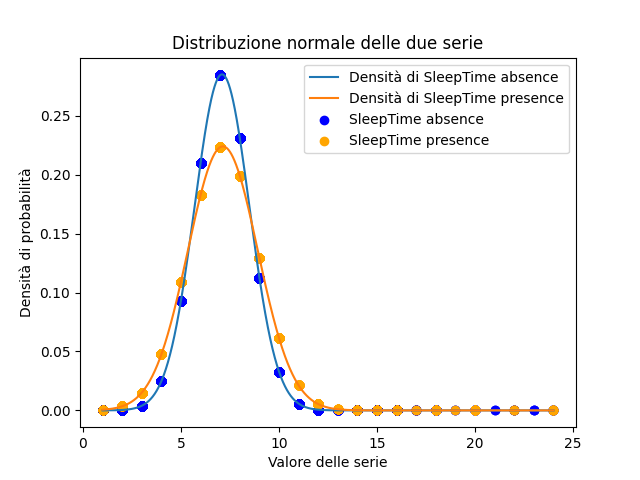
\includegraphics[width=0.75\linewidth]{TemplateTesi//immagini/sleeptimePKIdistr.png}
    \caption{Distribuzione della Feature 'SleepTime' in PKI}
    \label{fig:distrsleeppki}
\end{figure}

Ho calcolato lo score delle metriche per 
\newline
\emph{ChosenFeatures=[Age,Sex,Smoking,PhysicalActivity,GenHealth,DiffWalking]}
\newline
ottenendo:
\begin{lstlisting}
'test_accuracy': array([0.75085106, 0.75871825, 0.75833272, 0.75674467, 0.75738354]), 
'test_precision': array([0.72459836, 0.73654873, 0.73590252, 0.73289951, 0.7355619 ]), 
'test_recall': array([0.80928738, 0.80558547, 0.80587398, 0.80793662, 0.80370181])}
\end{lstlisting}
Dopo aver inserito tra le features scelte 'SleepTime', ottenendo così 
\newline
\emph{ChosenFeatures=[Age,Sex,Smoking,PhysicalActivity,GenHealth,DiffWalking,SleepTime]}

I risultati ottenuti sulle metriche sono i seguenti:

\begin{lstlisting}
'test_accuracy': array([0.75021448, 0.76433383, 0.7629009 , 0.76171223, 0.76186738]), 
'test_precision': array([0.73417613, 0.74445457, 0.74446236, 0.74511044, 0.74584433]), 
'test_recall': array([0.78445868, 0.80499425, 0.80061333, 0.79557154, 0.79446179])}
\end{lstlisting}

Anche in questo caso ho ottenuto un \emph{incremento globale di circa il 2\%}
\end{flushleft}


\subsection{Set di Feature Finali}
\begin{flushleft}
    
Dopo tali test sono stati creati per tutti i dataset i set di feature finali, qui riportati:

PKI:
\begin{lstlisting}
    Chosen_Features= ['Age','Sex','Smoking','PhysicalActivity','GenHealth','DiffWalking','PhysicalHealth','SleepTime']

\end{lstlisting}
HDD:
\begin{lstlisting}
Chosen_Features = ['Age', 'Sex', 'chest_pain_type', 'st_depression', 'st_slope', 'exercise_angina','Cholesterol','MaxHR']
\end{lstlisting}
    
UCI (uguali a quelli iniziali, non avendo effettuato la feature selection):

\begin{lstlisting}
Chosen_Features=['Age', 'Sex', 'chest_pain_type', 'st_depression', 'st_slope', 'exercise_angina','trestbps','Cholesterol,'fasting_blood_sugar','MaxHR','exercise_angina','vessel_fluoroscopy']
\end{lstlisting}
\end{flushleft}

\subsection{Sbilanciamento dei dataset} 
Nella seguente sezione saranno riportate le considerazioni effettuate e le tecniche utilizzate per il bilanciamento su tutti i dataset.
\newline
\textbf{PKI sbilanciato}
\begin{flushleft}
    
Nel caso di PKI, ho invididuato, come precedentemente menzionato un forte sbilanciamento  nella rappresentazione dei valori della feature target "Heart\_Disease". La classe che rappresentava l'assenza di problemi cardiaci era sovrarappresentata rispetto alla classe per la presenza. Per affrontare questo problema, ho attuato due tecniche di bilanciamento, ovvero SMOTE, per l' undersampling e ENN per l'oversampling.  

%Applicando entrambe le tecniche , sono stato in grado di ottenere un dataset  bilanciato, con una rappresentazione più equilibrata delle classi target. Questo ha fornito un set di dati più performante durante  l'addestramento e la valutazione dei modelli di ML selezionati.



Durante l'undersampling la classe maggioritaria è stata ridotta alla dimensione di quella minoritaria, invece durante oversampling la classe minoritaria è stata augmentata per raggiungere la numerosità di quella maggioritaria. I parametri con i quali sono state utilizzate tali tecniche sono "$sampling\_strategy=minority$" per SMOTE e "$n\_neighbour=3$" per ENN.
I risultati ottenuti sulle metriche saranno descritti nel paragrafo \ref{sec:risultati}.  %4.3. 
\newline
\textbf{HDD e UCI bilanciati}
\newline


Nel caso del dataset HDD e del dataset UCI, ho osservato che i dataset erano già bilanciati( come evidenziato nelle figure \ref{fig:istoHDDtarget} e \ref{fig:istoUCItarget}). Pertanto, non ho applicato  tecniche di bilanciamento, poiché i dataset stessi presentavano una rappresentazione equilibrata della classe target.



\section{Risultati finali per i modelli di classificazione }\label{sec:risultati}

Nella sezione seguente, verranno illustrate le tecniche impiegate sui tre dataset utilizzati per generare i modelli. Ogni dataset è stato sottoposto a tecniche diverse in base alle analisi presentate nelle sezioni precedenti. Per il dataset UCI abbiamo scelto di minimizzare l'insieme di tecniche usate, per osservare il comportamento del modello in questo caso. Successivamente, verranno presentate le metriche dei modelli completati. 
È fondamentale sottolineare che ogni risultato esposto in questa sezione rappresenta la media dei risultati ottenuti attraverso la cross-validation, garantendo così una buona valutazione dell'abilità di generalizzazione degli stessi.
I set di feature utilizzati durante questa fase sono quelli finali esposti in \ref{selezionesetfinali}.

Per ognuno dei 3 dataset considerati, sarà analizzato il comportamento del modello mediante la variazione del set di tecniche utilizzate. In particolare, si esaminerà l'impatto dell'esclusione di una specifica tecnica dal set completo di tecniche impiegate. Riporteremo quindi i risultati ottenuti utilizzando l'intero set di tecniche, ad eccezione di quella specifica tecnica in questione, come indicato chiaramente nelle tabelle e nei grafici (ad esempio quelli in figura \ref{fig:andamentometrichePKI} e \ref{fig:graficoandamentoPKI}).

\subsection{Tecniche Utilizzate}


\textbf{Tecniche applicate ad UCI:}
\begin{itemize}
    \item Manipolazioni (Sostituzione variabili nominali, rimozione NaN)
    \item Scaling dei Dati
\end{itemize}




\begin{figure}[H]
    \centering
    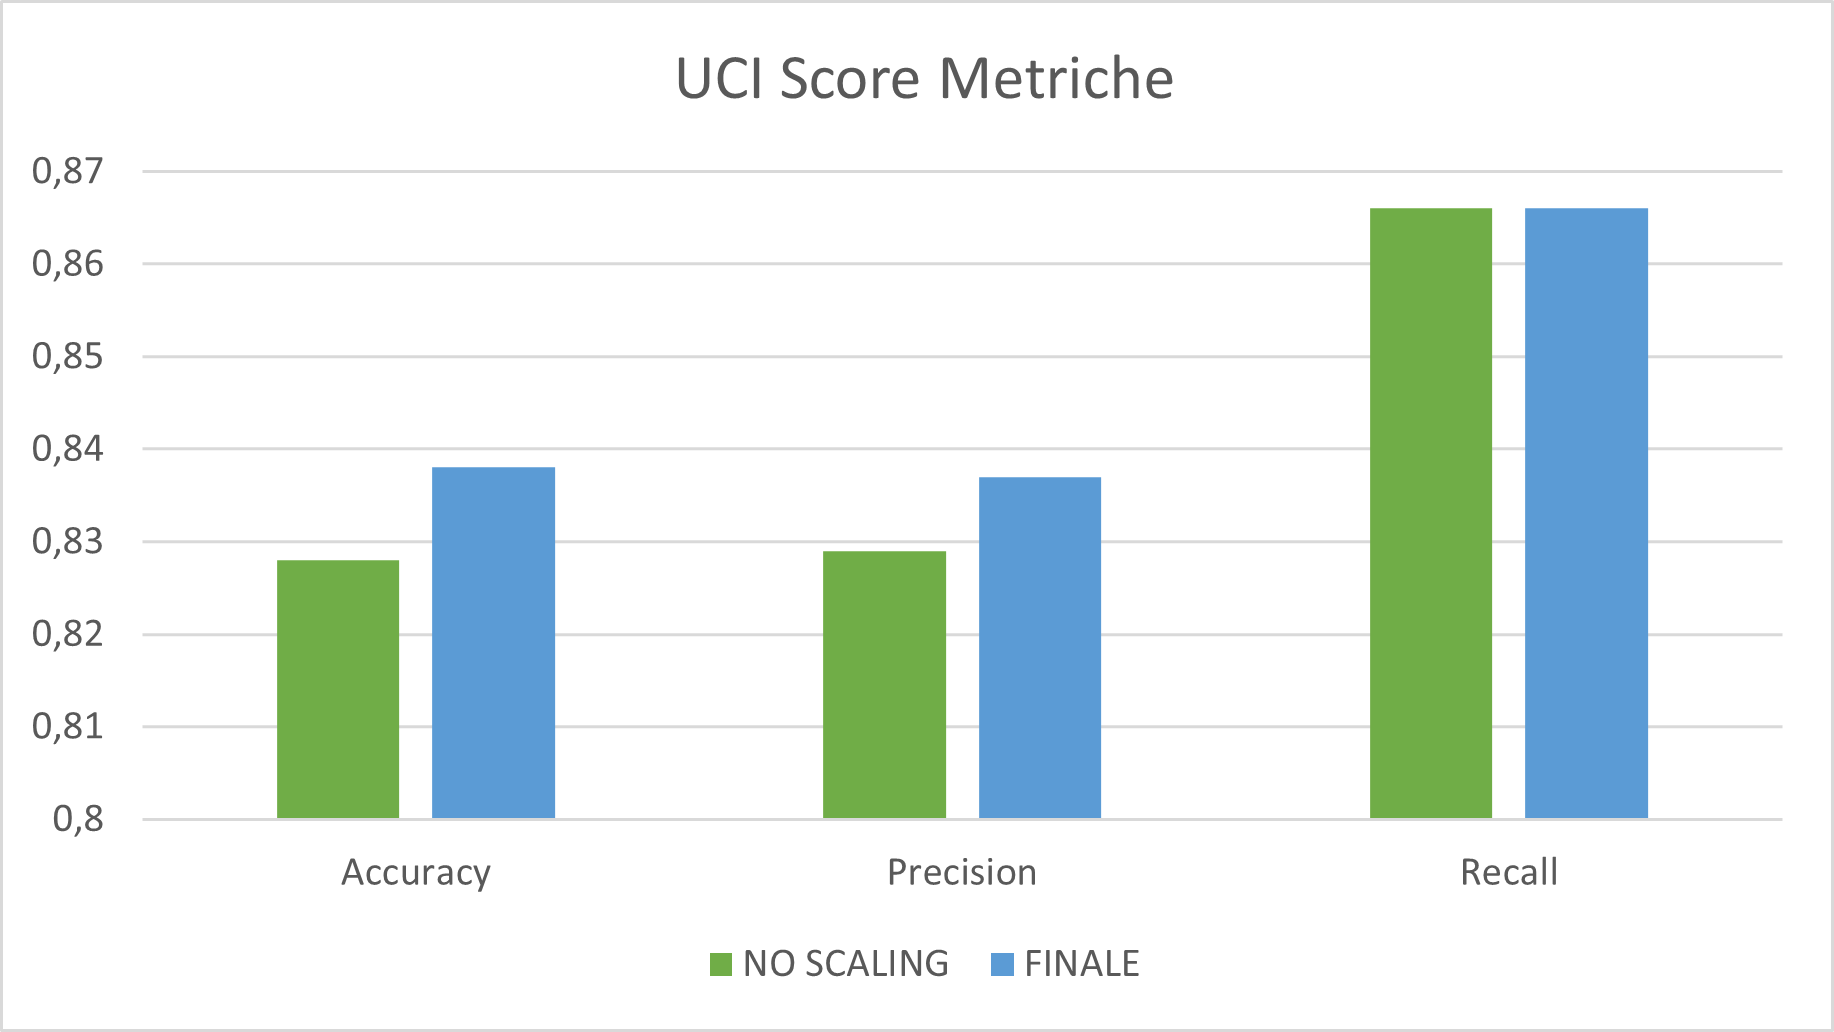
\includegraphics[width=0.75\linewidth]{TemplateTesi//immagini/graficoUCIMetriche.png}
    \caption{Grafico Dell'Andamento delle Metriche Relative al Dataset UCI}
    \label{fig:graficoandamentoUCI}
\end{figure}

I risultati ottenuti, visibili in figura \ref{fig:graficoandamentoUCI}, mostrano che l'uso dello scaling delle feature porta ad un leggero miglioramento delle metriche del modello, sebbene l'aumento sia modesto. Questo indica che l'applicazione dello scaling comunque contribuisce a una migliore normalizzazione dei dati consentendo al modello di lavorare in modo più efficace e coerente con i dati stessi.


\textbf{Tecniche applicate ad HDD:}
\begin{itemize}
    \item Feature Selection
    \item Manipolazioni (Sostituzione variabili nominali, rimozione NaN)
    \item Scaling dei Dati
    \item Rimozione deglia outlier: Zscore
\end{itemize}




\begin{figure}[H]
    \centering
    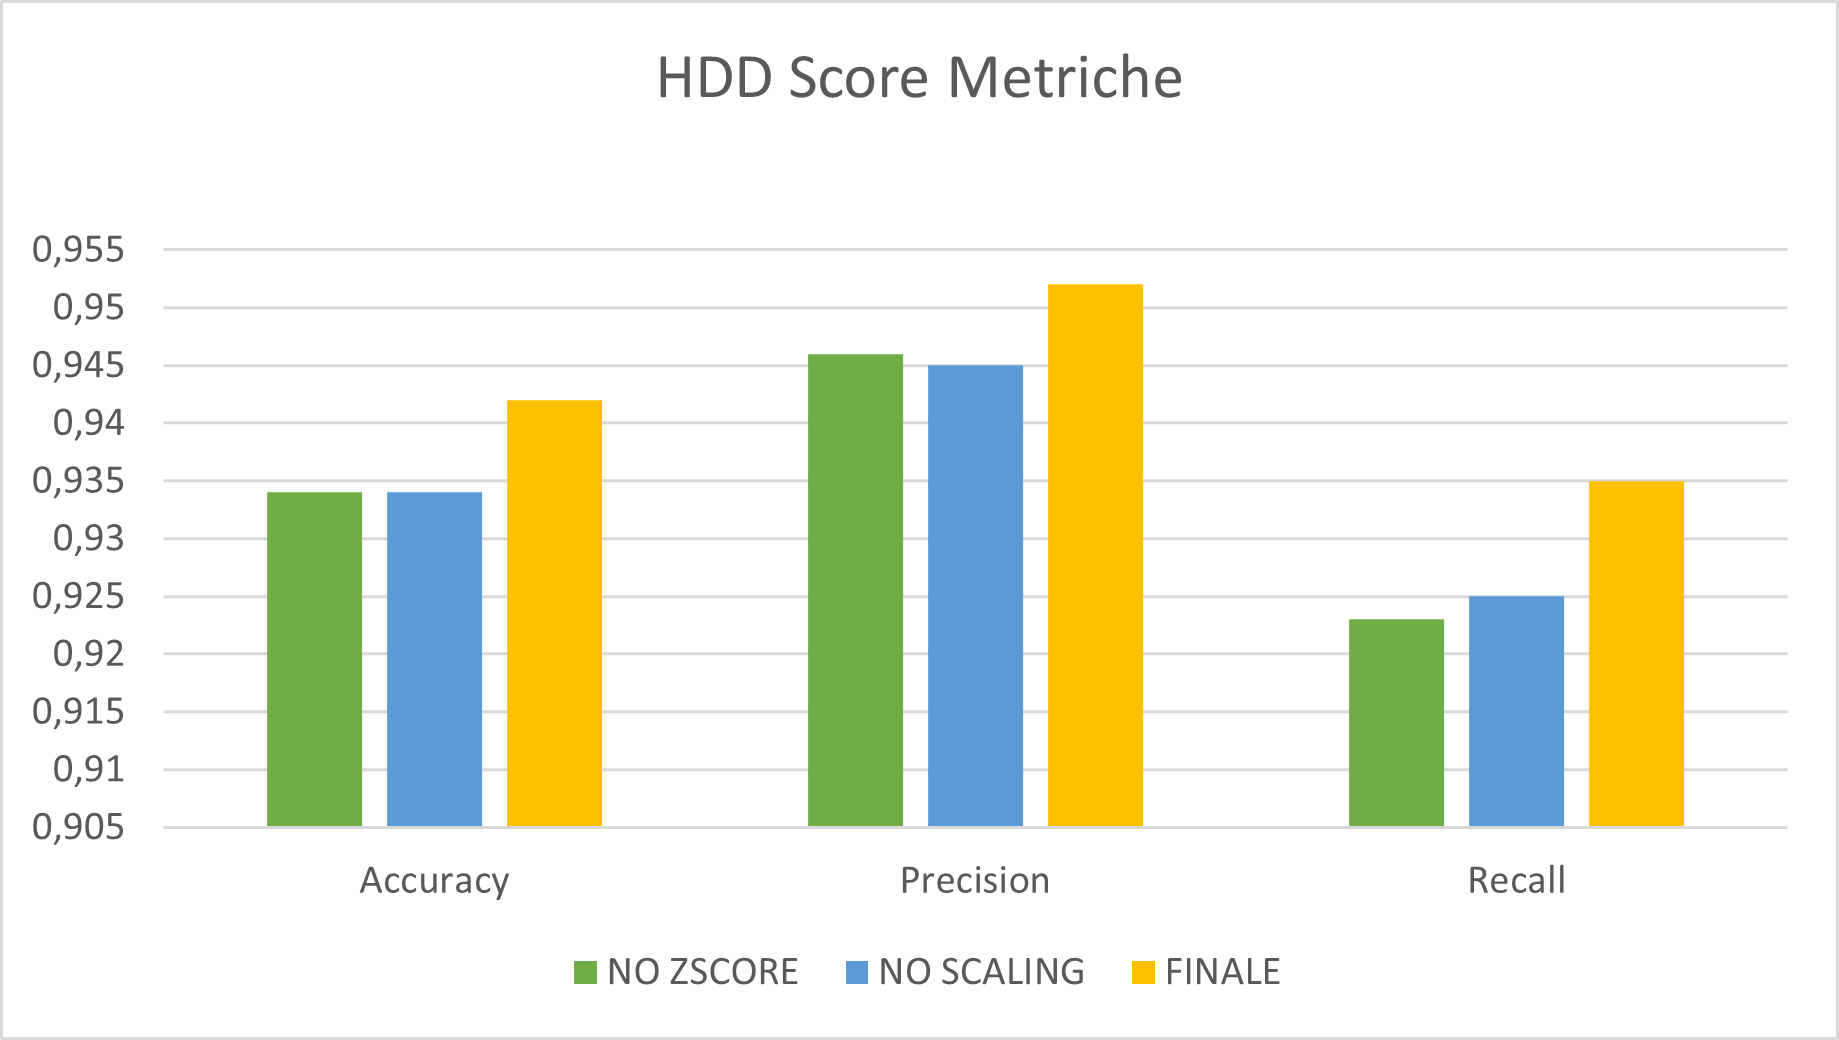
\includegraphics[width=0.75\linewidth]{TemplateTesi//immagini/graficoHDDMetriche.png}
    \caption{Grafico dell'Andamento delle Metriche Relative al Dataset HDD}
    \label{fig:graficoandamentoHDD}
\end{figure}

Anche in questo caso i risultati (in figura \ref{fig:graficoandamentoHDD}) hanno evidenziato che l'uso dello scaling delle feature porta ad un leggero miglioramento delle metriche del modello, così come il trattamento degli outlier con Z-score. Sebbene l'aumento non sia particolarmente alto singolarmente, si osserva che con l'uso di entrambe le tecniche vi è un aumento di circa 1 punto percentuale in tutte le metriche considerate. Sebbene possa sembrare un incremento modesto, specialmente in ambito clinico, rappresenta comunque un aiuto sostanzioso per il modello.

\textbf{Tecniche applicate a PKI:}
\begin{itemize}
    \item Feature Selection
    \item Manipolazioni (Sostituzione variabili nominali, rimozione NaN)
    \item Scaling dei Dati
    \item Rimozione outlier: Zscore
    \item SMOTE
    \item ENN
\end{itemize}


\begin{figure}[H]
    \centering
    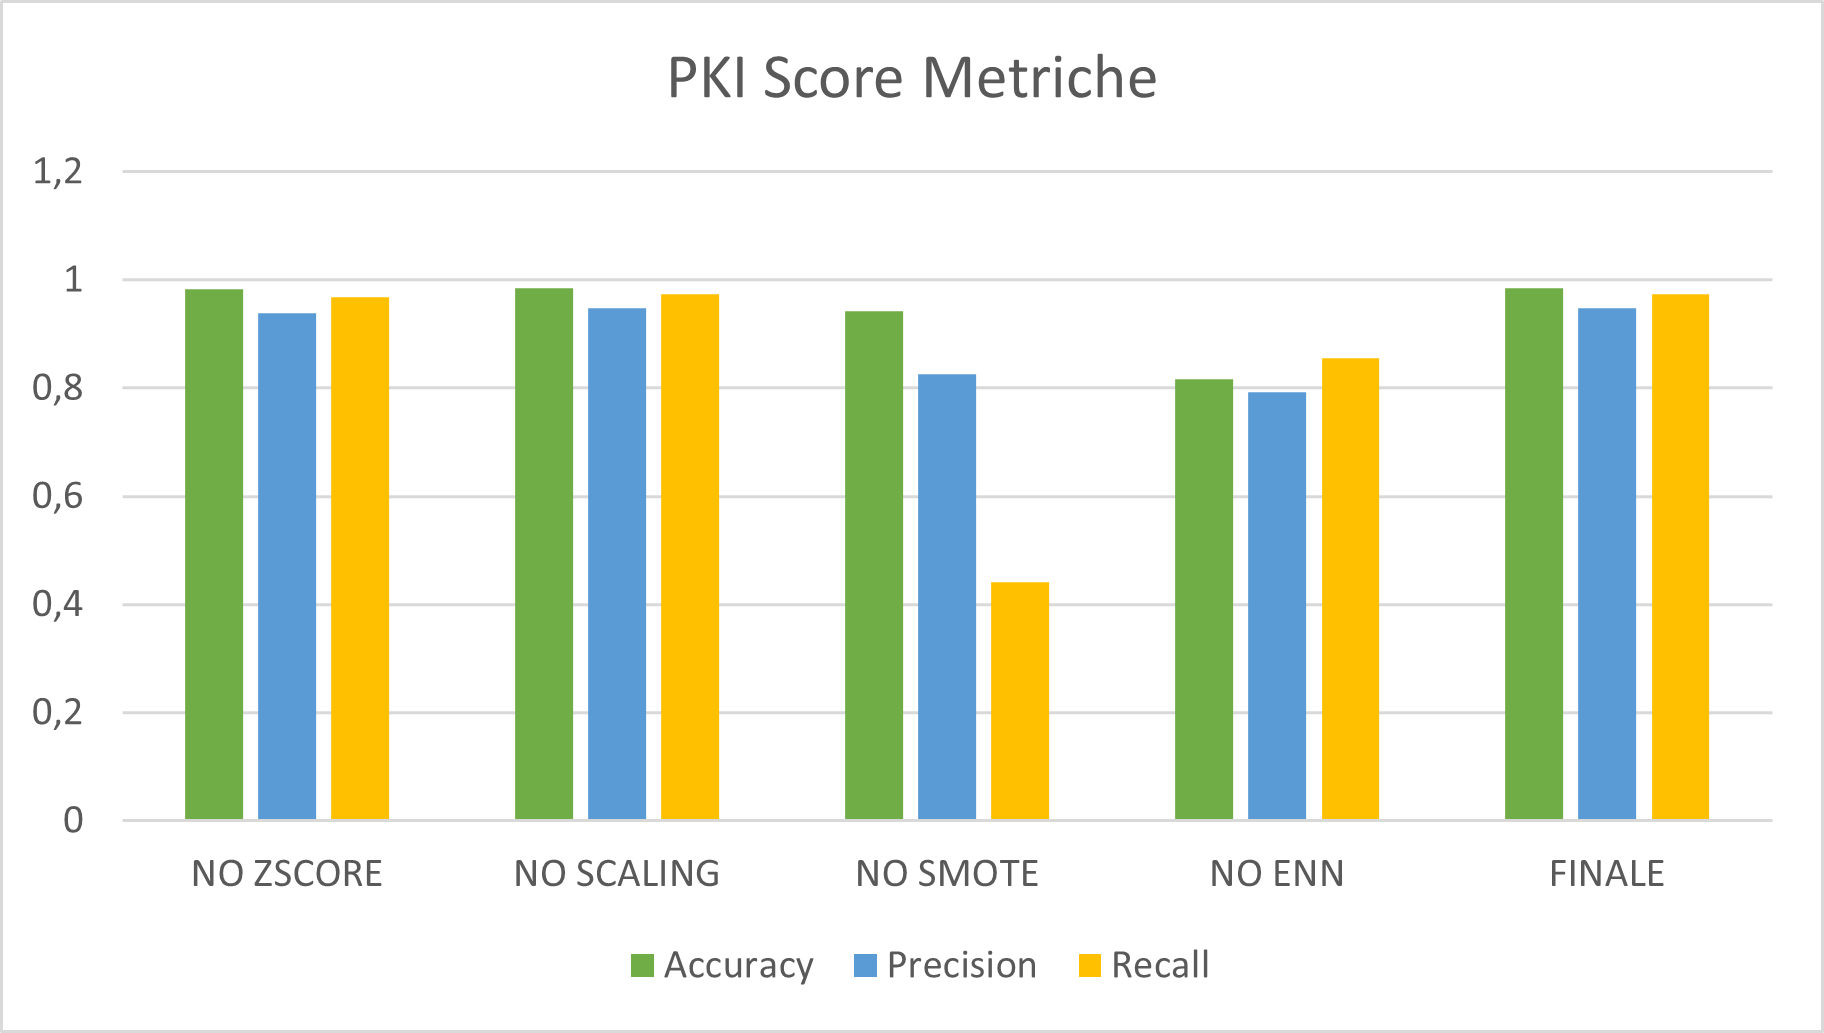
\includegraphics[width=0.75\linewidth]{TemplateTesi//immagini/graficoPKIMetriche.png}
    \caption{Grafico dell'Andamento delle Metriche Relative al Dataset PKI}
    \label{fig:graficoandamentoPKI}
\end{figure}
Analogamente a quanto verificato in precedenza si nota un aumento modesto delle metriche  con il trattamento degli outlier e lo scaling.

Un nuovo aspetto emerso dalle  analisi in figura \ref{fig:graficoandamentoPKI} riguarda l'utilizzo delle tecniche di bilanciamento come SMOTE e ENN. Data la presenza di uno sbilanciamento significativo nel dataset, queste tecniche hanno avuto un impatto estremamente significativo sulle performance del modello. In particolare, si è notato che l'applicazione di SMOTE ha influenzato in modo molto elevato la metrica di recall, evidenziando l'importanza di gestire il problema dello sbilanciamento per una classificazione accurata.


\newline
\textbf{Risultati finali:}
\newline
Dopo aver esaminato l'andamento delle metriche relative ai 3 modelli, è giunto il momento di esporre i risultati finali ottenuti su questi ultimi.

Questi risultati rappresentano una valutazione delle prestazioni dei modelli sviluppati e forniscono un'indicazione del loro livello di accuratezza e affidabilità.
I risultati finali costituiscono un importante contributo a questa tesi. Questi risultati forniscono una base per ulteriori ricerche e sviluppi nel campo del progetto in cui è calato il mio lavoro.
\begin{figure}[H]
    \centering
    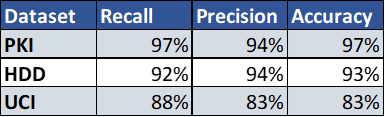
\includegraphics[width=0.55\linewidth]{TemplateTesi//immagini/MetricheModelliFinali.png}
    \caption{Metriche Finali Calcolate per i 3 Dataset}
    \label{fig:metrichefinali}
\end{figure}

Come evidenziato in figura \ref{fig:metrichefinali}, i punteggi delle metriche riflettono l'efficacia dei modelli costruiti.

Come prevedibile, il modello addestrato sul dataset UCI, che prevedeva meno elaborazioni, ha mostrato risultati inferiori rispetto agli altri modelli. Tuttavia, questi risultati sono comunque accettabili e non eccessivamente bassi, tenendo conto della complessità del problema e delle limitazioni sulle tecniche impiegate imposte da me.

Sono particolarmente soddisfatto dei risultati ottenuti per gli altri due modelli, i quali hanno raggiunto punteggi molto elevati nelle metriche considerate. Questo è particolarmente significativo nel contesto clinico, poiché stiamo lavorando con dati relativi ai pazienti e la precisione delle previsioni riveste un ruolo di grande importanza.

I punteggi così elevati sono a mio avviso specialmente importanti per il dataset PKI. Questo dataset, come spiegato in precedenza, si basa in gran parte su feature di tipo "personale", dove non è necessariamente richiesta la supervisione diretta di un esperto medico. Ciò si traduce in un notevole risparmio di tempo e risorse finanziarie per il settore medico, rendendo questo approccio al ML in ambito clinico a mio avviso prezioso.
\end{flushleft}

\section{XAI}
\begin{flushleft}
    
Nella seguente sezione sarà fornito un esempio di come sono state utilizzate le tecniche di Explainable Artificial Intelligence per fornire interpretazioni e spiegazioni comprensibili dei modelli creati durante il tirocinio.

Data la natura delle feature di tipo clinico utilizzate nei dataset, è di particolare importanza garantire la trasparenza sulle decisioni prese dal modello costruito.
A titolo esemplificativo, verranno illustrate le tecniche di XAI utilizzate durante l'analisi del dataset HDD, che contiene parametri clinici.

\subsection{LIME}
Utilizzando LIME, sono stato in grado di identificare le caratteristiche cliniche che hanno avuto un impatto significativo sulle decisioni prese dal modello, tale tecnica risulta di particolare interesse quando il risultato fornito riguarda un caso liminare della classificazione.
Un esempio di visualizzazione per un caso liminare  è fornito in figura \ref{fig:LimeLiminare}.

\begin{figure}[H]
    \centering
    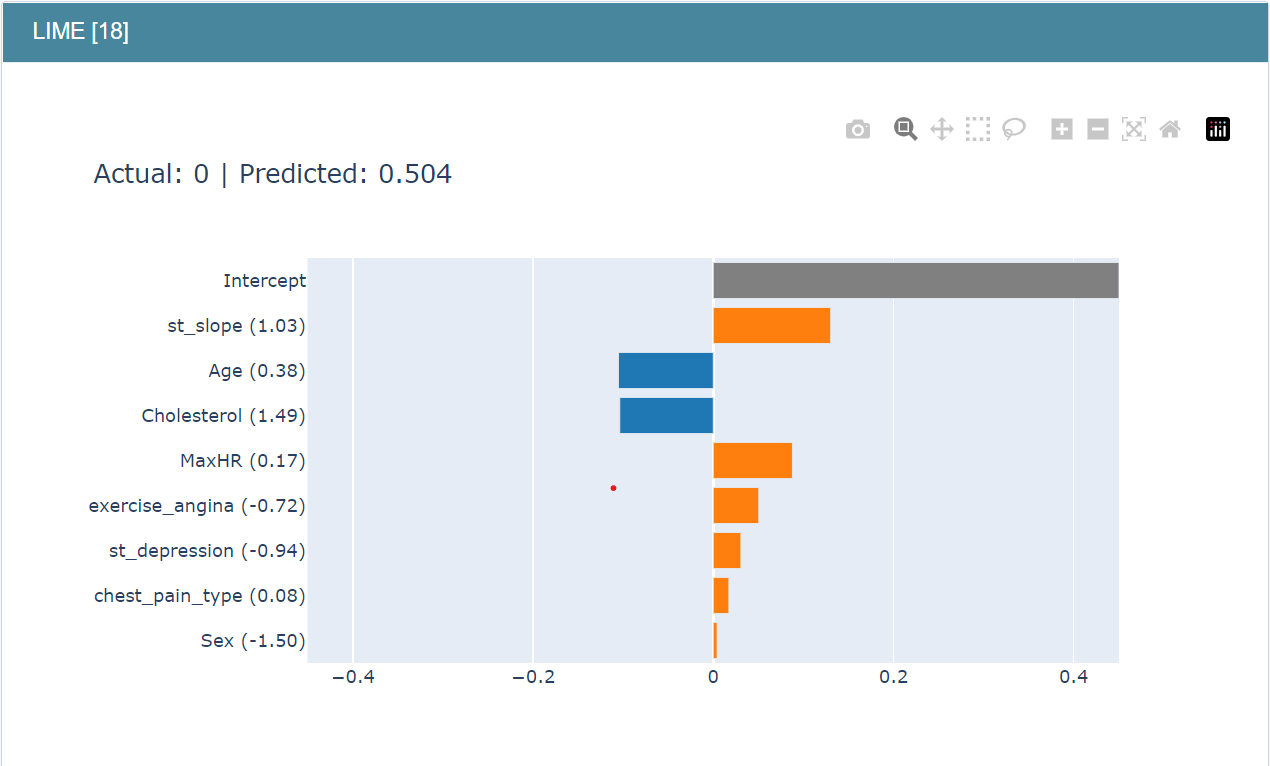
\includegraphics[width=1\linewidth]{TemplateTesi//immagini/casoliminare.png}
    \caption{Esempio di Visualizzazione LIME per un caso liminare}
    \label{fig:LimeLiminare}
\end{figure}

L'analisi dei risultati ottenuti mediante il grafico generato da LIME ha rivelato che la feature ST slope ha avuto il maggior impatto sulla classificazione del paziente come nella classe "0" (sena malattia). Questo indica come la feature "St slope" possa essere un elemento rilevante al fine della decisione nel nostro problema di classificazione.

Si osserva come l'età e il colesterolo abbiano hanno contribuito in senso opposto rispetto alla classificazione, in contrasto con ST slope e il resto delle feature.


Le considerazioni derivate da quest'analisi offrono alla figura medica uno strumento  per un'interpretazione più approfondita dei risultati delle previsioni.
Questo può fornire inoltre una nuova prospettiva clinica e rappresentare un caso di studio per un approccio personalizzato al trattamento dei pazienti.

\subsection{Counterfactual Explanations}


Nella seguente sezione si riportano le counterfactual explanations generate per un particolare record.
Nel suddetto caso il record ( la prima riga in figura \ref{fig:exCF}), rappresenta una paziente (poiché la feature Sex=1) con un'età di 57 anni e la presenza di malattie cardiovascolari (Heart Disease=1).

\begin{figure}[H]
    \centering
    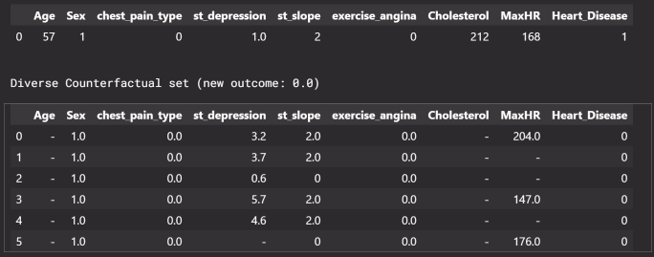
\includegraphics[width=1\linewidth]{TemplateTesi//immagini/CFexample.png}
    \caption{Esempio di Visualizzazione delle Counterfactual Explanations}
    \label{fig:exCF}
\end{figure}

Per questo esempio, nel processo di generazione delle counterfactual explanations, ho  deciso di consentire  possibili modifiche solo sulle feature specifiche di ST depression, ST slope, "exercise angina" e "max HR", mantenendo le altre feature fisse. Questa scelta è stata effettuata per fornire un esempio tecnico di come le modifiche a queste feature possono influenzare la classificazione del modello. 

È importante sottolineare che le modifiche apportate alle feature durante la creazione delle counterfactual explanations siano puramente a scopo illustrativo dal punto di vista tecnico. È fondamentale che i range di valori modificabili delle feature siano supervisionate e valutate da un esperto clinico, in base alle sue considerazioni mediche e al contesto del paziente.
 
Si riportano quindi le variazioni effettuate dalla tecnica:

Complessivamente, sono state generate 6 counterfactual explanations.  I risultati ci mostrano come sia stato suggerito di aumentare la ST depression in 4 casi su 6, indicando che un aumento della depressione del tratto ST può potenzialmente influire fortemente sulla classificazione del modello, permettendo di cambiare alla fine la classe del paziente.
La feature ST slope è stata variata solo in due delle 6 spiegazioni generate, con una diminuzione suggerita in entrambi i casi.

La feature "exercise angina" è rimasta invariato in tutte le spiegazioni, suggerendo che la presenza o l'assenza di angina indotta dall'esercizio fisico non ha influenzato la classificazione nel nostro caso specifico.
La feature "max HR" è stata variata 3 volte, con alcune spiegazioni che suggerivano un aumento e altre un decremento del battito cardiaco massimo.
